\documentclass[a4paper]{article}
\let\Tiny=\tiny
% Included packages ---------------------------------------------------------- %
\usepackage{inputenc}                 % utf-8 encoding, æ, ø , å, etc.
\usepackage{a4wide}                          % Adjust margins to better fit A4 format.
\usepackage{array}                           % Matrices.
\usepackage{amsmath}                         % Math symbols, and enhanced matrices.
\usepackage{amsfonts}                        % Math fonts.
\usepackage{amssymb}                         % Additional symbols.
\usepackage{wasysym}                         % More additional symbols.
\usepackage{mathrsfs}                        % Most additional symbols.
\usepackage[pdftex]{graphicx}                % Improved inclusion of .pdf-graphics files.
\usepackage{sidecap}                         % Floats with captions to the right/left.
\usepackage{cancel}                          % Visualize cancellations in equations.
\usepackage{enumerate}                       % Change counters (arabic, roman, etc.).
\usepackage{units}                           % Adds better looking fractions (nicefrac).
\usepackage{floatrow}                        % Multi-figure floats.
\usepackage{subfig}                          % Multi-figure floats.
\usepackage{caption}                         % Adds functionality to captions.
\usepackage{bm}                              % Bolded text in math mode.
\usepackage{combinedgraphics}                % Figures; let latex handle the text itself.
\usepackage[framemethod=default]{mdframed}   % Make boxes.
\usepackage{listings}                        % For including source code.
\usepackage[colorlinks]{hyperref}            % Interactive references, colored.
\usepackage{soul}                            % Make vertical bars through text.
\usepackage{nicefrac}                        % Nice fractions with \nicefrac.
\usepackage{mathtools}                       % Underbrackets, overbrackets.
\usepackage{wasysym}                         % \smiley{}-s!
\usepackage{multicol}                        % Multiple text columns.
\usepackage{capt-of}                         % Caption things which are not floats.
\usepackage[url=false]{biblatex}             % Citations (made easy).
\usepackage{simplewick}                      % Contractions using Wick's theorem for QFT.
\usepackage{booktabs}                        % Tables.
\usepackage{bbold}
\usepackage{tikz}

% Differentials -------------------------------------------------------------- %
\newcommand{\dt}{\,\mathrm{d}t}
\newcommand{\dx}{\,\mathrm{d}x}
\newcommand{\dr}{\,\mathrm{d}r}

% Derivatives ---------------------------------------------------------------- %
\newcommand{\der} [2]{\frac{\mathrm{d} #1}{\mathrm{d} #2}}   % Derivative.
\newcommand{\pder}[2]{\frac{\partial #1}{\partial #2}}       % Partial derivative.

% Matrices ------------------------------------------------------------------- %
\newcommand{\mat} [2]{\begin{matrix}[#1] #2 \end{matrix}}    % Nothing enclosing it.
\newcommand{\pmat}[2]{\begin{pmatrix}[#1] #2 \end{pmatrix}}  % Enclosing parentheses.
\newcommand{\bmat}[2]{\begin{bmatrix}[#1] #2 \end{bmatrix}}  % Enclosing square brackets.
\newcommand{\vmat}[2]{\begin{vmatrix}[#1] #2 \end{vmatrix}}  % Enclosing vertical bars.
\newcommand{\Vmat}[2]{\begin{Vmatrix}[#1] #2 \end{Vmatrix}}  % Enclosing double bars.

% Number sets ---------------------------------------------------------------- %
\newcommand{\R}{\mathbb{R}}
\newcommand{\Q}{\mathbb{Q}}
\newcommand{\N}{\mathbb{N}}
\newcommand{\Z}{\mathbb{Z}}
\newcommand{\C}{\mathbb{C}}

% Manually set alignment of rows / columns in matrices (mat, pmat, etc.) ----- %
\makeatletter
\renewcommand*\env@matrix[1][*\c@MaxMatrixCols c]{%
  \hskip -\arraycolsep
  \let\@ifnextchar\new@ifnextchar
  \array{#1}}
\makeatother

% References ----------------------------------------------------------------- %
\newcommand{\Fig}[1]{Fig.\ \ref{fig:#1}}
\newcommand{\fig}[1]{Fig.\ \ref{fig:#1}}
\newcommand{\eq} [1]{Eq.\ (\ref{eq:#1})}
\newcommand{\Eq} [1]{Eq.\ (\ref{eq:#1})}
\newcommand{\tab}[1]{Table \ref{tab:#1}}
\newcommand{\Tab}[1]{Table \ref{tab:#1}}

% Paragraph formatting ------------------------------------------------------- %
\setlength{\parindent}{5.5mm}
\setlength{\parskip}  {0mm}

% Source code listings ------------------------------------------------------- %
\definecolor{commentGreen}{RGB}{34,139,34}
\definecolor{keywordBlue}{RGB}{0,0,255}
\definecolor{stringPurple}{RGB}{160,32,240}
\lstset{language=matlab}
\lstset{basicstyle=\ttfamily\small}
\lstset{frame=single}
\lstset{stringstyle=\color{stringPurple}}
\lstset{keywordstyle=\color{keywordBlue}}
\lstset{commentstyle=\color{commentGreen}}
\lstset{morecomment=[l][\color{commentGreen}\bfseries]{\%\%}}
\lstset{showspaces=false}
\lstset{showstringspaces=false}
\lstset{showtabs=true}
\lstset{columns=fixed}
\lstset{breaklines}
\lstset{literate={~} {$\sim$}{1}}
\lstset{numbers=left}              
\lstset{stepnumber=1}
\renewcommand{\ttdefault}{pcr}
\lstdefinestyle{prt}{frame=none,basicstyle=\ttfamily\small}

% Convenient shorthand notation ---------------------------------------------- %
\newcommand{\nn}{\nonumber}
\newcommand{\e}[1]{\cdot10^{#1}}
\renewcommand{\i}{\hat{\imath}}
\renewcommand{\j}{\hat{\jmath}}
\renewcommand{\k}{\hat{k}}

% Caption position of tables at the top -------------------------------------- %
\floatsetup[table]{capposition=top}

% Black frame with white background ------------------------------------------ %
\newmdenv[linecolor=black,backgroundcolor=white]{exframe}

% Including vector drawings from inkscape ------------------------------------ %
\newenvironment{combFig}[5]{
  \begin{figure}[#1] 
    \centering 
    \includecombinedgraphics[vecscale=#2, keepaspectratio]{#3} 
    \caption{#4 \label{#5}}
  \end{figure}
  }

  {
}

% Including pdf graphics ----------------------------------------------------- %
\newenvironment{pdfFig}[5]{
  \begin{figure}[#1] 
    \centering 
    \includegraphics[width= #2]{#3} 
    \caption{#4 \label{#5}}
  \end{figure}
  }

  {
}

% Exercise and subexercise counters ------------------------------------------ %
\newcounter{excounter}
\renewcommand\theexcounter{\arabic{excounter}}
\newcommand\exlabel{\theexcounter}
\setcounter{excounter}{1}

\newcounter{subexcounter}
\renewcommand\thesubexcounter{\arabic{subexcounter}}
\newcommand\subexlabel{\thesubexcounter}
\setcounter{subexcounter}{1}

% Environments for exercises ------------------------------------------------- %
\newenvironment{exercise}[1]{
  \subsection*{Exercise \theexcounter: #1}
  \setcounter{subexcounter}{1}                      % Reset the subexercise counter to a.
  \addcontentsline{toc}{section}{\theexcounter: #1} % Add the exercise to TOC
  }
      % Exercise text.
  {
  \stepcounter{excounter}                           % Add one to the exercise counter.
  \newpage
}

% Environment for subexercises ----------------------------------------------- %
\newenvironment{subexercise}{
  \begin{exframe}
    \begin{itemize}  \setlength{\itemindent}{1cm}
      \item[{\bf Exercise \thesubexcounter}] 
	}
	  % Subexercise text.
	{
    \end{itemize}
  \end{exframe}
  \stepcounter{subexcounter}                        % Add one to the exercise counter.
}

% Environment for proofs ----------------------------------------------------- %
\newenvironment{proof}[2]{
  \begin{exframe}
    \begin{itemize}  \setlength{\itemindent}{0.6cm}
      \item[{\bf #1} {\bf #2}] 
	}
	  % Subexercise text.
	{
    \end{itemize}
  \end{exframe}
}

% Environment for answers ---------------------------------------------------- %
\newenvironment{answer}{}{}

% Set bibliography file and path for images.
\bibliography{references/fys4180ref.bib}
\graphicspath{{./images/}}
\newcommand{\includepdfgraphics}[2]{\includecombinedgraphics[#1]{./images/#2}}



\renewcommand{\L}{\hat{L}_z}
\renewcommand{\S}{\hat{S}_z}
\newcommand{\slater}{|P_1P_2\dots P_N\rangle}
\newcommand{\cm}{c_\mu}
\newcommand{\cn}{c_\nu}
\newcommand{\cmd}{c_\mu^\dagger}
\newcommand{\cnd}{c_\nu^\dagger}
\newcommand{\ca}{c_\alpha}
\newcommand{\cad}{c_\alpha^\dagger}
\newcommand{\cb}{c_\beta}
\newcommand{\cbd}{c_\beta^\dagger}

\renewcommand{\u}[1]{{\bf #1}_\uparrow}
\renewcommand{\d}[1]{{\bf #1}_\downarrow}

\newcommand{\boud}{b_{\u{1}}^\dagger}
\newcommand{\bou}{b_{\u{1}}}
\newcommand{\bodd}{b_{\d{1}}^\dagger}
\newcommand{\bod}{b_{\d{1}}}

\newcommand{\bfud}{b_{\u{5}}^\dagger}
\newcommand{\bfu}{b_{\u{5}}}
\newcommand{\bfdd}{b_{\d{5}}^\dagger}
\newcommand{\bfd}{b_{\d{5}}}

\newcommand{\ps}{{p\sigma}}
\newcommand{\cpp}{c_{p+}}
\newcommand{\cppd}{c_{p+}^\dagger}
\newcommand{\cpm}{c_{p-}}
\newcommand{\cpmd}{c_{p-}^\dagger}
\newcommand{\cqp}{c_{q+}}
\newcommand{\cqpd}{c_{q+}^\dagger}
\newcommand{\cqm}{c_{q-}}
\newcommand{\cqmd}{c_{q-}^\dagger}
\newcommand{\crp}{c_{r+}}
\newcommand{\crpd}{c_{r+}^\dagger}
\newcommand{\crm}{c_{r-}}
\newcommand{\crmd}{c_{r-}^\dagger}

% Title
\title{FYS-KJM4480 Project 2}
\date{}
\author{Morten Ledum}
% ---------------------------------------------------------------------------- %
% ---------------------------------------------------------------------------- %
\begin{document}
\maketitle
\subsection*{Exercise 1}

\begin{exframe}
We define first 
\begin{align}
\hat H = \hat H_0 + \hat V = \sum_{p\sigma} \epsilon_p c_\ps^\dagger c_\ps - \sum_{pq}\frac{1}{2}g \cpp^\dagger \cpm^\dagger \cqm \cqp,
\end{align}
with the ground state wave function of $\hat H_0$ being the Slater determinant (for the $N=4$ particles case) 
\begin{align}
|\Phi\rangle = c_{1+}^\dagger c_{1-}^\dagger c_{2+}^\dagger c_{2-}^\dagger |-\rangle.
\end{align}
The pair creation and annihilation operators are defined as follows
\begin{align}
\hat P^\dagger_p \equiv \cpp^\dagger \cpm^\dagger, \ \ \ \text{ and } \ \ \ \hat P_p \equiv \cpm \cpp,
\end{align}
with the number operator, the pair-number operator, and the spin-projection operators defined as
\begin{align}
\hat n_p \equiv \sum_\sigma c_\ps^\dagger c_\ps, \ \ \ \hat P \equiv \sum_p \hat P^\dagger_p \hat P_p, \ \ \ \text{ and } \ \ \ \hat S_z \equiv \frac{1}{2}\sum_\ps \sigma c_\ps^\dagger c_\ps.
\end{align}
\begin{itemize}
  \item[a)] Show that $\hat H_0$ and $\hat V$ commute with $\hat S_z$.
\end{itemize}
\end{exframe}
From the definitions of $\hat H_0$ and $\hat S_z$ we find that
\begin{align}
\hat H_0 \hat S_z &= \left(  \sum_\ps \epsilon_p c_\ps^\dagger c_\ps \right) \left(   \frac{1}{2}\sum_{p'\sigma'} \sigma' c_{p'\sigma'}^\dagger c_{p'\sigma'}  \right) \nn\\
%
&= \frac{1}{2}\sum_\ps \sum_{p'\sigma'}\sigma'  \epsilon_p c_\ps^\dagger c_\ps  c_{p'\sigma'}^\dagger c_{p'\sigma'} \nn\\
%
&= \frac{1}{2}\sum_\ps \sum_{p'\sigma'}\sigma'  \epsilon_p c_\ps^\dagger c_\ps  c_{p'\sigma'}^\dagger c_{p'\sigma'}.
\end{align}
Let us consider the operator string, and begin our long journey of anti-commuting things with
\begin{align}
c_\ps^\dagger c_\ps  c_{p'\sigma'}^\dagger c_{p'\sigma'} &= c_\ps^\dagger (-c_{p'\sigma'}^\dagger c_\ps   + \delta_{p\sigma p'\sigma'}) c_{p'\sigma'} \nn\\
%
&= c_{p'\sigma'}^\dagger c_\ps^\dagger  c_\ps c_{p'\sigma'}   + \delta_{p\sigma p'\sigma'}c_\ps^\dagger c_{p'\sigma'} \nn\\
%
&= -c_{p'\sigma'}^\dagger c_\ps^\dagger c_{p'\sigma'} c_\ps    + c_\ps^\dagger c_{p\sigma} \nn\\
%
&= -c_{p'\sigma'}^\dagger (- c_{p'\sigma'}c_\ps^\dagger + \delta_{p\sigma p'\sigma'}) c_\ps    + c_\ps^\dagger c_{p\sigma} \nn\\
%
&= c_{p'\sigma'}^\dagger c_{p'\sigma'}c_\ps^\dagger c_\ps -   \delta_{p\sigma p'\sigma'} c_{p'\sigma'}^\dagger c_\ps   + c_\ps^\dagger c_{p\sigma} \nn\\
%
&= c_{p'\sigma'}^\dagger c_{p'\sigma'}c_\ps^\dagger c_\ps -   c_{p\sigma}^\dagger c_\ps   + c_\ps^\dagger c_{p\sigma} \nn\\
%
&= c_{p'\sigma'}^\dagger c_{p'\sigma'}c_\ps^\dagger c_\ps,
\end{align}
where we have used the fundamental anti-commutation relations multiple times. We note that we have now switched the orders of $\hat H_0$ and $\hat S_z$, meaning that $\hat H_0 \hat S_z = \hat S_z \hat H_0$, i.e. the commutator vanishes.

We continue with $\hat V$ and $\hat S_z$, and find that
\begin{align}
\hat V \hat S_z &= \left(   - \sum_{pq}\frac{1}{2}g \cpp^\dagger \cpm^\dagger \cqm \cqp   \right)  \left(   \frac{1}{2}\sum_{p'\sigma'} \sigma' c_{p'\sigma'}^\dagger c_{p'\sigma'}  \right) \nn\\ 
%
&= -\frac{1}{4}\sum_{pq}\sum_{p'\sigma'}g\sigma' \cpp^\dagger \cpm^\dagger \cqm \cqp  c_{p'\sigma'}^\dagger c_{p'\sigma'},
\end{align}
from which we extract the operator string and compute
\begin{align}
\cpp^\dagger \cpm^\dagger \cqm \cqp  c_{p'\sigma'}^\dagger c_{p'\sigma'} &= \cpp^\dagger \cpm^\dagger \cqm (-  c_{p'\sigma'}^\dagger \cqp + \delta_{p'\sigma'q+}) c_{p'\sigma'} \nn\\
%
&= -\cpp^\dagger \cpm^\dagger  \cqm c_{p'\sigma'}^\dagger \cqp c_{p'\sigma'} + \cpp^\dagger \cpm^\dagger \cqm  \cqp \nn\\
%
&= -\cpp^\dagger \cpm^\dagger (- c_{p'\sigma'}^\dagger \cqm + \delta_{p'\sigma'q-}) \cqp c_{p'\sigma'} + \cpp^\dagger \cpm^\dagger \cqm  \cqp \nn\\
%
&= \cpp^\dagger \cpm^\dagger c_{p'\sigma'}^\dagger \cqm \cqp c_{p'\sigma'} - \delta_{p'\sigma'q-} \cpp^\dagger \cpm^\dagger \cqp c_{p'\sigma'}  + \cpp^\dagger \cpm^\dagger \cqm  \cqp \nn\\
%
&= c_{p'\sigma'}^\dagger \cpp^\dagger \cpm^\dagger \cqm \cqp c_{p'\sigma'} -  \cpp^\dagger \cpm^\dagger \cqp \cqm  + \cpp^\dagger \cpm^\dagger \cqm  \cqp \nn\\
%
&= c_{p'\sigma'}^\dagger \cpp^\dagger \cpm^\dagger c_{p'\sigma'} \cqm \cqp   + 2\cpp^\dagger \cpm^\dagger \cqm  \cqp \nn\\
%
&= c_{p'\sigma'}^\dagger \cpp^\dagger(-c_{p'\sigma'} \cpm^\dagger +\delta_{p'\sigma' p-}) \cqm \cqp   + 2\cpp^\dagger \cpm^\dagger \cqm  \cqp \nn\\
%
&= -c_{p'\sigma'}^\dagger \cpp^\dagger c_{p'\sigma'} \cpm^\dagger \cqm \cqp +\delta_{p'\sigma' p-} c_{p'\sigma'}^\dagger \cpp^\dagger \cqm \cqp  + 2\cpp^\dagger \cpm^\dagger \cqm  \cqp \nn\\
% 
&= -c_{p'\sigma'}^\dagger (- c_{p'\sigma'} \cpp^\dagger + \delta_{p'\sigma'p+}) \cpm^\dagger \cqm \cqp + \cpm^\dagger \cpp^\dagger \cqm \cqp  + 2\cpp^\dagger \cpm^\dagger \cqm  \cqp \nn\\
%
&= c_{p'\sigma'}^\dagger c_{p'\sigma'} \cpp^\dagger \cpm^\dagger \cqm \cqp - \delta_{p'\sigma'p+}c_{p'\sigma'}^\dagger \cpm^\dagger \cqm \cqp - \cpp^\dagger \cpm^\dagger  \cqm \cqp  + 2\cpp^\dagger \cpm^\dagger \cqm  \cqp \nn\\
%
&= c_{p'\sigma'}^\dagger c_{p'\sigma'} \cpp^\dagger \cpm^\dagger \cqm \cqp - \cpp^\dagger \cpm^\dagger \cqm \cqp + \cpp^\dagger \cpm^\dagger \cqm  \cqp \nn\\
%
&= c_{p'\sigma'}^\dagger c_{p'\sigma'} \cpp^\dagger \cpm^\dagger \cqm \cqp.
\end{align}
Fortunately, we note that we have again switched the order of the operators, meaning $[\hat V, \hat S_z]=0$ as expected.

\begin{exframe}
\begin{itemize}
  \item[b)] Show that $\hat H_0$ and $\hat V$ commute with $\hat P$.
\end{itemize}
\end{exframe}
Again, we simply insert the definitions and start anti-commuting operators past each other. Doing this yields
\begin{align}
 \hat P \hat H_0 &= \left(  \sum_p \hat P^\dagger_p \hat P_p\right) \left(  \sum_{p'\sigma'} \epsilon_{p'} c_{p'\sigma'}^\dagger c_{p'\sigma'} \right) \nn\\
%
&= \left(  \sum_p \cpp^\dagger \cpm^\dagger \cpm \cpp \right) \left(  \sum_{p'\sigma'} \epsilon_{p'} c_{p'\sigma'}^\dagger c_{p'\sigma'} \right)  \nn\\
%
&= \sum_p \sum_{p'\sigma'} \epsilon_{p'} \cpp^\dagger \cpm^\dagger \cpm \cpp   c_{p'\sigma'}^\dagger c_{p'\sigma'} \nn\\
%
&= -\sum_p \sum_{p'\sigma'} \epsilon_{p'} \cpp^\dagger \cpm^\dagger \cpp \cpm   c_{p'\sigma'}^\dagger c_{p'\sigma'},  \footnote{Note the minus sign (I had the wrong definitions of the $\hat P$ operator while typing this in, and didnt feel like redoing everything up to \eq{1} so I snuck in a sign change here).}
\end{align}
with
\begin{align}
\cpp^\dagger \cpm^\dagger \cpp \cpm c_{p'\sigma'}^\dagger c_{p'\sigma'} &= \cpp^\dagger \cpm^\dagger \cpp (-c_{p'\sigma'}^\dagger \cpm + \delta_{p'\sigma' p-}) c_{p'\sigma'} \nn\\
%
&= -\cpp^\dagger \cpm^\dagger \cpp c_{p'\sigma'}^\dagger \cpm c_{p'\sigma'}  + \delta_{p'\sigma' p-}  \cpp^\dagger \cpm^\dagger \cpp c_{p'\sigma'} \nn\\
%
&= -\cpp^\dagger \cpm^\dagger (-c_{p'\sigma'}^\dagger \cpp + \delta_{p'\sigma'p+}) \cpm c_{p'\sigma'}  +  \cpp^\dagger \cpm^\dagger \cpp \cpm \nn\\
%
&= \cpp^\dagger \cpm^\dagger c_{p'\sigma'}^\dagger \cpp \cpm c_{p'\sigma'}  - \delta_{p'\sigma'p+}\cpp^\dagger \cpm^\dagger \cpm c_{p'\sigma'}  +  \cpp^\dagger \cpm^\dagger \cpp \cpm \nn\\
%
&= c_{p'\sigma'}^\dagger \cpp^\dagger \cpm^\dagger \cpp \cpm c_{p'\sigma'}   - \cpp^\dagger \cpm^\dagger \cpm \cpp +  \cpp^\dagger \cpm^\dagger \cpp \cpm \nn\\
%
&= c_{p'\sigma'}^\dagger \cpp^\dagger \cpm^\dagger c_{p'\sigma'} \cpp \cpm    + \cpp^\dagger \cpm^\dagger \cpp \cpm  +  \cpp^\dagger \cpm^\dagger \cpp \cpm \nn\\
%
&= c_{p'\sigma'}^\dagger \cpp^\dagger \cpm^\dagger c_{p'\sigma'} \cpp \cpm    + \cpp^\dagger \cpm^\dagger \cpp \cpm  +  \cpp^\dagger \cpm^\dagger \cpp \cpm \nn\\
%
&= c_{p'\sigma'}^\dagger \cpp^\dagger (-c_{p'\sigma'}\cpm^\dagger + \delta_{p'\sigma'p-}) \cpp \cpm   +  2\cpp^\dagger \cpm^\dagger \cpp \cpm \nn\\
%
&= -c_{p'\sigma'}^\dagger \cpp^\dagger c_{p'\sigma'}\cpm^\dagger \cpp \cpm + \delta_{p'\sigma'p-} c_{p'\sigma'}^\dagger \cpp^\dagger  \cpp \cpm   +  2\cpp^\dagger \cpm^\dagger \cpp \cpm \nn\\
%
&= -c_{p'\sigma'}^\dagger (-c_{p'\sigma'}\cpp^\dagger +\delta_{p'\sigma'p+}) \cpm^\dagger \cpp \cpm + \cpm^\dagger \cpp^\dagger  \cpp \cpm   +  2\cpp^\dagger \cpm^\dagger \cpp \cpm \nn\\
%
&= c_{p'\sigma'}^\dagger c_{p'\sigma'}\cpp^\dagger \cpm^\dagger \cpp \cpm - \delta_{p'\sigma'p+} c_{p'\sigma'}^\dagger \cpm^\dagger \cpp \cpm - \cpp^\dagger\cpm^\dagger  \cpp \cpm   +  2\cpp^\dagger \cpm^\dagger \cpp \cpm \nn\\
%
&= c_{p'\sigma'}^\dagger c_{p'\sigma'}\cpp^\dagger \cpm^\dagger \cpp \cpm - \cpp^\dagger \cpm^\dagger \cpp \cpm  +  \cpp^\dagger \cpm^\dagger \cpp \cpm \nn\\
%
&= c_{p'\sigma'}^\dagger c_{p'\sigma'}\cpp^\dagger \cpm^\dagger \cpp \cpm. \label{eq:1}
\end{align}
As before, we note that we have switched the order of the operators and thus the commutator $[\hat H_0,\hat P]=0$.

%Moving on now, I grow bored with typing all of this in (and I assume no one is going to bother reading it in detail anyway), so we the following we use some tricks. The first of which is noting that for a general Slater determinant $|\Psi\rangle = c_{i\sigma_i}^\dagger c_{j\sigma_j}^\dagger c_{k\sigma_k}^\dagger \dots c_{j\sigma_j}^\dagger |-\rangle$, operating with $\hat V$ involves doing 
%\begin{align}
%\hat V |\Psi\rangle = \sum_{pq}-\frac{1}{2}g \cpp^\dagger \cpm^\dagger \cqm \cqp |\Psi\rangle.
%\end{align}
%We note that the only way to get a non-zero result from the terms in the sum is to demand that $p+$ and $p-$ \emph{are} in $|\Psi\rangle$, while $q+$ and $q-$ are \emph{not}. But this means that we annihilate and create one particle with spin projection $\sigma=+$ (the $c_{p+}^\dagger$ and $c_{q+}$ operators) and we annihilate and create one particle with spin projection $\sigma=-$ (the $c_{p-}^\dagger$ and $c_{q-}$ operators). Thus the total spin projection of $|\Phi\rangle$ does not change under $\hat V$, and so it does not matter if we apply $\hat S_z$ before or after $\hat V$. 

Moving on, we consider the $\hat V \hat P$, and find
\begin{align}
\hat V \hat P &= \left(  \sum_{pq} -\frac{1}{2}g \cppd \cpmd \cqm \cqp \right) \left( \sum_r \crpd \crmd \crm \crp \right) \nn\\
%
&= -\frac{1}{2}g\sum_{pq}\sum_r \cppd \cpmd \cqm \cqp \crpd \crmd \crm \crp,
\end{align}
with
\begin{align}
\cppd \cpmd \cqm \cqp \crpd \crmd \crm \crp &= \cppd \cpmd \cqm (-\crpd\cqp  + \delta_{r+q+}) \crmd \crm \crp \nn\\
%
&= -\cppd \cpmd \cqm\crpd\cqp \crmd \crm \crp +  (\delta_{r+q+}) \cppd \cpmd \cqm \crmd \crm \crp \nn\\
%
&= -\cppd \cpmd (-\crpd\cqm + \delta_{r+q-})\cqp \crmd \crm \crp + A \nn\\
%
&= \cppd \cpmd \crpd\cqm \cqp \crmd \crm \crp - (\delta_{r+q-})\cppd \cpmd \cqp \crmd \crm \crp + A \nn\\
%
&= \crpd \cppd \cpmd \cqm \cqp \crmd \crm \crp + B \nn\\
%
&= \crpd \cppd \cpmd \cqm (- \crmd\cqp + \delta_{r-q+}) \crm \crp + B \nn\\
%
&= -\crpd \cppd \cpmd \cqm \crmd\cqp \crm \crp + (\delta_{r-q+}) \crpd \cppd \cpmd \cqm \crm \crp   + B \nn\\
%
&= -\crpd \cppd \cpmd (- \crmd\cqm + \delta_{r-q-})\cqp \crm \crp + C \nn\\
%
&= \crpd \cppd \cpmd \crmd\cqm \cqp \crm \crp - (\delta_{r-q-})\crpd \cppd \cpmd \cqp \crm \crp+ C \nn\\
%
&= \crpd \cppd \cpmd \crmd\cqm \cqp \crm \crp + D \nn\\
%
&= \crpd \crmd \cppd \cpmd \crm \cqm \cqp  \crp + D \nn\\
%
&= \crpd \crmd \cppd (- \crm\cpmd + \delta_{r-p-}) \cqm \cqp  \crp + D \nn\\
%
&= -\crpd \crmd \cppd \crm\cpmd  \cqm \cqp  \crp + (\delta_{r-p-}) \crpd \crmd \cppd\cqm \cqp  \crp + D \nn
\end{align}
\begin{align}
&= -\crpd \crmd \cppd \crm\cpmd  \cqm \cqp  \crp + E \nn\\
%
&= -\crpd \crmd (- \crm\cppd + \delta_{r-p+}) \cpmd  \cqm \cqp  \crp + E \nn\\
%
&= \crpd \crmd \crm\cppd \cpmd  \cqm \cqp  \crp - (\delta_{r-p+})\crpd \crmd \cpmd  \cqm \cqp  \crp + E \nn\\
%
&= \crpd \crmd \crm\cppd \cpmd \crp \cqm \cqp   + F \nn\\
%
&= \crpd \crmd \crm\cppd (- \crp\cpmd +\delta_{r+p-}) \cqm \cqp   + F \nn\\
%
&= -\crpd \crmd \crm\cppd \crp\cpmd \cqm \cqp + (\delta_{r+p-})\crpd \crmd \crm\cppd \cqm \cqp    + F \nn\\
%
&= -\crpd \crmd \crm(- \crp\cppd + \delta_{r+p+})\cpmd \cqm \cqp + G \nn\\
%
&= \crpd \crmd \crm \crp\cppd \cpmd \cqm \cqp - (\delta_{r+p+})\crpd \crmd \crm \cpmd \cqm \cqp + G \nn\\
%
&= \crpd \crmd \crm \crp\cppd \cpmd \cqm \cqp + H,
\end{align}
with the constants $A$ through $G$ defined as 
\begin{align}
A &\equiv \phantom{A - }\,\,(\delta_{r+q+}) \cppd \cpmd \cqm \crmd \crm \crp, \\
B &\equiv A - (\delta_{r+q-})\cppd \cpmd \cqp \crmd \crm \crp, \\
C &\equiv B + (\delta_{r-q+}) \crpd \cppd \cpmd \cqm \crm \crp, \\
D &\equiv C - (\delta_{r-q-})\crpd \cppd \cpmd \cqp \crm \crp, \\
E &\equiv D + (\delta_{r-p-}) \crpd \crmd \cppd\cqm \cqp  \crp, \\
F &\equiv E - (\delta_{r-p+})\crpd \crmd \cpmd  \cqm \cqp  \crp, \\
G &\equiv F + (\delta_{r+p-})\crpd \crmd \crm\cppd \cqm \cqp, \ \ \text{and}\\
H &\equiv G - (\delta_{r+p+})\crpd \crmd \crm \cpmd \cqm \cqp.
\end{align}
Showing that $H$ vanishes (the first and second cancel the seventh and eight, and the third through the sixth cancel each other) is left as an exercise for the reader (because frankly I grow bored with this, and I doubt you will even more than glance at these equations). 

We note that this shows $\hat V \hat P=\hat P \hat V$ and thus the commutator vanishes.

\begin{exframe}
\begin{itemize}
  \item[c)] Show that $\hat P$ commutes with $\hat S_z$.
\end{itemize}
\end{exframe}
Once again, from the definitions, we find
\begin{align}
\hat P \hat S_z &= \left( \sum_r \crpd \crmd \crm \crp \right) \left( \frac{1}{2}\sum_\ps \sigma c_\ps^\dagger c_\ps  \right) \nn\\
%
&= \frac{1}{2}\sum_r \sum_\ps  \sigma \crpd \crmd \crm \crp  c_\ps^\dagger c_\ps,
\end{align}
with
\begin{align}
\crpd \crmd \crm \crp  c_\ps^\dagger c_\ps &= \crpd \crmd \crm (-c_\ps^\dagger \crp + \delta_{p\sigma r+}) c_\ps \nn\\
%
&= -\crpd \crmd \crm c_\ps^\dagger \crp c_\ps + \delta_{p\sigma r+} \crpd \crmd \crm c_\ps \nn\\
%
&= -\crpd \crmd (- c_\ps^\dagger \crm + \delta_{p\sigma r-})\crp c_\ps +  \crpd \crmd \crm \crp \nn\\
%
&= \crpd \crmd c_\ps^\dagger \crm \crp c_\ps -  \delta_{p\sigma r-}\crpd \crmd\crp c_\ps + \crpd \crmd \crm \crp \nn\\
%
&= c_\ps^\dagger\crpd \crmd  \crm \crp c_\ps -  \crpd \crmd\crp \crm - \crpd \crmd \crp\crm  \nn\\
%
&= c_\ps^\dagger\crpd \crmd c_\ps  \crm \crp  -  2\crpd \crmd \crp\crm  \nn\\
%
&= c_\ps^\dagger\crpd ( c_\ps \crmd + \delta_{p\sigma r-})  \crm \crp  -  2\crpd \crmd \crp\crm  \nn\\
%
&= -c_\ps^\dagger\crpd  c_\ps \crmd \crm \crp + \delta_{p\sigma r-}c_\ps^\dagger\crpd  \crm \crp -  2\crpd \crmd \crp\crm  \nn
\end{align}
\begin{align}
&= -c_\ps^\dagger (- c_\ps\crpd + \delta_{p\sigma r+}) \crmd \crm \crp + \crmd\crpd  \crm \crp -  2\crpd \crmd \crp\crm  \nn\\
%
&= c_\ps^\dagger c_\ps\crpd \crmd \crm \crp - \delta_{p\sigma r+} c_\ps^\dagger\crmd \crm \crp + \crpd\crmd   \crp\crm -  2\crpd \crmd \crp\crm  \nn\\
%
&= c_\ps^\dagger c_\ps\crpd \crmd \crm \crp -  \crpd\crmd \crm \crp - \crpd \crmd \crp\crm  \nn\\
%
&= c_\ps^\dagger c_\ps\crpd \crmd \crm \crp +  \crpd\crmd \crp\crm  - \crpd \crmd \crp\crm  \nn\\
%
&= c_\ps^\dagger c_\ps\crpd \crmd \crm \crp.
\end{align}
We note that we have switched the order of operators and found equality, meaning the commutator must again vanish.
\begin{exframe}
\begin{itemize}
  \item[d)] Show that $[\hat P_p, \hat P_q^\dagger] = \delta_{pq}(1-\hat n_q).$
\end{itemize}
\end{exframe}
For the last time now (thankfully!) we begin from the definitions and find that
\begin{align}
\hat P_p \hat P_q^\dagger &= \cpm \cpp \cqpd \cqmd \nn\\
%
&= \cpm (-\cqpd\cpp + \delta_{q+p+}) \cqmd \nn\\
%
&= -\cpm \cqpd\cpp \cqmd + \delta_{q+p+} \cpm\cqmd \nn\\
%
&= -(- \cqpd\cpm + \delta_{q+p-})\cpp \cqmd + \delta_{q+p+} \cpm\cqmd \nn\\
%
&= \cqpd\cpm \cpp \cqmd - \delta_{q+p-}\cpp \cqmd + \delta_{q+p+} \cpm\cqmd \nn\\
%
&= \cqpd\cpm (-\cqmd\cpp + \delta_{q-p+}) - \delta_{q+p-}\cpp \cqmd + \delta_{q+p+} \cpm\cqmd \nn\\
%
&= -\cqpd\cpm \cqmd\cpp + \delta_{q-p+}\cqpd\cpm - \delta_{q+p-}\cpp \cqmd + \delta_{q+p+} \cpm\cqmd \nn\\
%
&= -\cqpd(- \cqmd\cpm + \delta_{q-p-})\cpp + \delta_{q-p+}\cqpd\cpm - \delta_{q+p-}\cpp \cqmd + \delta_{q+p+} \cpm\cqmd \nn\\
%
&= \cqpd\cqmd\cpm \cpp - \delta_{q-p-} \cqpd\cpp+ \delta_{q-p+}\cqpd\cpm - \delta_{q+p-}\cpp \cqmd + \delta_{q+p+} \cpm\cqmd \nn\\
&= \hat P_q^\dagger \hat P_p - \delta_{q-p-} \cqpd\cpp+ \delta_{q-p+}\cqpd\cpm - \delta_{q+p-}\cpp \cqmd + \delta_{q+p+} \cpm\cqmd. \label{eq:2}
\end{align}
Let us in more detail consider the extra four terms which have appeared in \eq{2}:
\begin{align}
- \delta_{q-p-} \cqpd\cpp&+ \delta_{q-p+}\cqpd\cpm - \delta_{q+p-}\cpp \cqmd + \delta_{q+p+} \cpm\cqmd \nn\\
&= - \delta_{qp}\delta_{--} \cqpd\cpp+ \delta_{qp}\delta_{-+}\cqpd\cpm - \delta_{qp}\delta_{+-}\cpp \cqmd + \delta_{qp}\delta_{++} \cpm\cqmd \nn\\
%
&= - \delta_{qp} \cqpd\cpp+  \delta_{qp} \cpm\cqmd \nn\\
%
&= \delta_{qp}\left(\cpm\cqmd  -\cqpd\cpp \right)\nn\\
%
&= \delta_{qp}\left(-\cqmd\cpm + \delta_{p-q-}  -\cqpd\cpp \right)\nn\\
%
&= \delta_{qp}\left(-\cqmd\cpm + \delta_{pq}\delta_{--}  -\cqpd\cpp \right)\nn\\
%
&= \delta_{qp}\left(\delta_{pq} -\cqmd\cpm  -\cqpd\cpp \right) = \delta_{pq}\left(\delta_{pq} - \hat n_q\right) = \delta_{pq}\left(1 - \hat n_q\right),
\end{align}
where we have used that the internal delta function just evaluates to one after evaluating the outer one. We note from this that $\hat P_p \hat P_q^\dagger = \hat P_q^\dagger \hat P_p + \delta_{pq} (1 - \hat n_p) \Rightarrow [\hat P_p, \hat P_q^\dagger] = \delta_{pq}(1-\hat n_p)$. 

\begin{exframe}
\begin{itemize}
  \item[e)] Show that $\hat P|\Phi\rangle=2|\Phi\rangle$, and that $\hat S_z|\Phi\rangle = 0 |\Phi\rangle$.
\end{itemize}
\end{exframe}
Restricting ourselves to the subspace of the total Hilbert space in which $P=2$, we note that we can write any Slater determinant as $|\Phi\rangle = |r\bar r s\bar s\rangle$, with $1 \le r,\bar r, s, \bar s \le 4$. The label $r,s$ denotes the $r/s$-th single particle orbital with positive spin-projection, while $\bar r, \bar s$ denotes the $r/s$-th single particle orbital with negative spin-projection.

Operating from the left with $\hat P$ on $|\Phi\rangle$ yields 
\begin{align}
\hat P |\Phi\rangle &= \sum_{p} \hat P_p^\dagger \hat P_p |\Phi\rangle \nn\\
%
&= \sum_{p} \cppd\cpmd \cpm \cpp |\Phi\rangle \nn\\ 
%
&= \sum_{p} \cppd\cpmd \cpm \cpp |r\bar r s \bar s\rangle.
\end{align}
Since operating on the Slater determinant with $\hat P_q=\cqm\cqp$ on $|\Phi\rangle$ yields $0$ unless a pair of $q$ states are in the determinant. This means 
\begin{align}
\hat P |\Phi\rangle &= \sum_{p} \cppd\cpmd \cpm \cpp |r\bar r s \bar s\rangle \nn\\
%
&= \crpd\crmd \crm \crp |r\bar r s \bar s\rangle + c_{s+}^\dagger c_{s-}^\dagger c_{s-} c_{s+} |r\bar r s \bar s\rangle \nn\\
%
&= |r\bar r s \bar s\rangle + |r\bar r s \bar s\rangle = 2|r\bar r s \bar s\rangle.
\end{align}

Moving on, we consider the action of $\hat S_z$ on $|\Phi\rangle$ and find
\begin{align}
\hat S_z |\Phi\rangle &= \frac{1}{2}\sum_\ps \sigma c_{p\sigma}^\dagger c_{p\sigma} |r\bar r s \bar s\rangle \nn\\
%
&= \frac{(-1)}{2} c_{r-}^\dagger c_{r-} |r\bar r s \bar s\rangle + \frac{(+1)}{2} c_{r+}^\dagger c_{r+} |r\bar r s \bar s\rangle + \frac{(-1)}{2} c_{s-}^\dagger c_{s-} |r\bar r s \bar s\rangle + \frac{(+1)}{2} c_{s+}^\dagger c_{s+} |r\bar r s \bar s\rangle \nn\\
&= \frac{1}{2}\left(1-1+1-1\right)  |r\bar r s \bar s\rangle = 0,
\end{align}
where all other $\ps$ combinations in the sum give zero since the Slater does not contain any of those orbitals. 

\begin{exframe}
\begin{itemize}
  \item[f)] Explain why the following set of Slater determinants form a basis for the subspace of Hilbert space with $S_z=0$ and $P=2$:
  \begin{align}
  |p\bar p q\bar q\rangle = \hat P_p^\dagger \hat P_q^\dagger |-\rangle, \ \ \ 1\le p<q\le M.
  \end{align}
  Here, $\bar p$ indicates the state $p-$, while $p$ indicates the state with $p+$. Draw spin-orbital diagrams for $M=4$ and label properly. Draw all the basis states. What is the dimension of the subspace (for arbitrary $M$)?
\end{itemize}
\end{exframe}
\begin{figure}
\begin{center}
  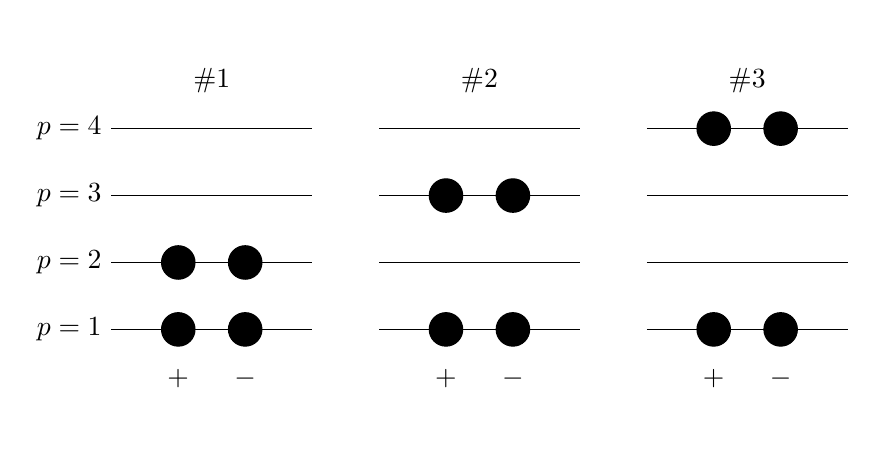
\begin{tikzpicture}[scale=0.85]
    \begin{scope}
      \foreach \i in {1,...,4}
      {
        \draw (-1,\i-1) node[anchor=east] {$p = \i$} --(2,\i-1);
      }
      \filldraw (0,0) node[anchor=north,inner sep=.5cm] {$+$} circle (0.25cm); 
      \filldraw (1,0) node[anchor=north,inner sep=.5cm] {$-$} circle (0.25cm);
      \filldraw (0,1) circle (0.25cm); 
      \filldraw (1,1) circle (0.25cm);
      \filldraw (0.5,4.5) node[anchor=north,inner sep=.5cm] {$\#1$} ; 
    \end{scope}
    \begin{scope}[xshift=4cm]
      \foreach \i in {1,...,4}
      {
        \draw (-1,\i-1) --(2,\i-1);
      }
      \filldraw (0,0) node[anchor=north,inner sep=.5cm] {$+$} circle (0.25cm); 
      \filldraw (1,0) node[anchor=north,inner sep=.5cm] {$-$} circle (0.25cm);
      \filldraw (0,2) circle (0.25cm); 
      \filldraw (1,2) circle (0.25cm);
      \filldraw (0.5,4.5) node[anchor=north,inner sep=.5cm] {$\#2$} ;
    \end{scope}
    \begin{scope}[xshift=8cm]
      \foreach \i in {1,...,4}
      {
        \draw (-1,\i-1) --(2,\i-1);
      }
      \filldraw (0,0) node[anchor=north,inner sep=.5cm] {$+$} circle (0.25cm); 
      \filldraw (1,0) node[anchor=north,inner sep=.5cm] {$-$} circle (0.25cm);
      \filldraw (0,3) circle (0.25cm); 
      \filldraw (1,3) circle (0.25cm);
      \filldraw (0.5,4.5) node[anchor=north,inner sep=.5cm] {$\#3$} ;
    \end{scope}
  \end{tikzpicture}
  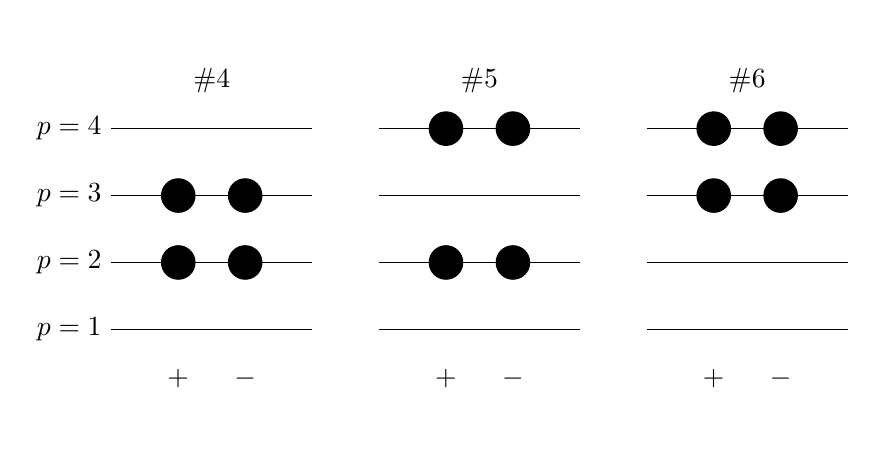
\begin{tikzpicture}[scale=0.85]
      \begin{scope}[xshift=0cm]
      \foreach \i in {1,...,4}
      {
        \draw (-1,\i-1) node[anchor=east] {$p = \i$} --(2,\i-1);
      }
      \filldraw (0,0) node[anchor=north,inner sep=.5cm] {$+$} ; 
      \filldraw (1,0) node[anchor=north,inner sep=.5cm] {$-$} ;
      \filldraw (0,1) circle (0.25cm); 
      \filldraw (1,1) circle (0.25cm); 
      \filldraw (0,2) circle (0.25cm); 
      \filldraw (1,2) circle (0.25cm);
      \filldraw (0.5,4.5) node[anchor=north,inner sep=.5cm] {$\#4$} ;
    \end{scope}
    \begin{scope}[xshift=4cm]
      \foreach \i in {1,...,4}
      {
        \draw (-1,\i-1) --(2,\i-1);
      }
      \filldraw (0,0) node[anchor=north,inner sep=.5cm] {$+$} ; 
      \filldraw (1,0) node[anchor=north,inner sep=.5cm] {$-$} ;
      \filldraw (0,1) circle (0.25cm); 
      \filldraw (1,1) circle (0.25cm); 
      \filldraw (0,3) circle (0.25cm); 
      \filldraw (1,3) circle (0.25cm);
      \filldraw (0.5,4.5) node[anchor=north,inner sep=.5cm] {$\#5$} ;
    \end{scope}
    \begin{scope}[xshift=8cm]
      \foreach \i in {1,...,4}
      {
        \draw (-1,\i-1) --(2,\i-1);
      }
      \filldraw (0,0) node[anchor=north,inner sep=.5cm] {$+$} ; 
      \filldraw (1,0) node[anchor=north,inner sep=.5cm] {$-$} ;
      \filldraw (0,3) circle (0.25cm); 
      \filldraw (1,3) circle (0.25cm); 
      \filldraw (0,2) circle (0.25cm); 
      \filldraw (1,2) circle (0.25cm);
      \filldraw (0.5,4.5) node[anchor=north,inner sep=.5cm] {$\#6$} ;
    \end{scope}
  \end{tikzpicture}
\end{center}
\caption{All the basis states in the subspace of the Hilbert space with $S_z=0$, $P=2$, $N=4$, and $M=4$. The states are arbitrarily assigned for all the states (except for the reference state which naturally is labeled with the index $1$). \label{fig:1}}
\end{figure}
Any state in the Hilbert space must have total spin zero, meaning that there must be an equal number of particles with positive spin-projection as there are with negative spin-projection. Also, we need the state to contain \emph{exactly} two pairs of particles in the $p-$ and $p+$ ($1\le p \le 4$) orbitals. Since the states represented in \fig{1} exhaust all possible states in the $M=N=4$ space under these constraints, we know that they form a basis for the space. Denoting these states by the numbers $I=1,2,\dots,6$, we note that they are orthogonal 
\begin{align}
\langle I | J \rangle &= \langle p\bar p q\bar q | r\bar r s\bar s\rangle = \delta_{pr}\delta_{\bar p \bar r}\delta_{qs}\delta_{\bar q \bar s}.
\end{align}

For $N=4$ with some $M\ge 2$, finding the number of total basis functions is a simple combinatorics problem. There are $M$ possible pair levels, and two pairs to place. The number of unique ways of distributing $2$ pairs across $M$ possible levels is $M$ choose $2$, i.e.
\begin{align}
\text{basis size} = {M\choose2} = \frac{M!}{2!(M-2)!}.
\end{align}
A few examples of the basis size are $M=4$: $6$, $M=10$: $45$, and $M=100$: $4950$. We note that in the general case, with no restrictions on $S_z$ and $P$, the entire Hilbert space will have 
\begin{align}
\text{basis size}_\text{general} = {2M\choose4},
\end{align}
e.g. $70$ for the $M=4$ case.

\begin{exframe}
\begin{itemize}
  \item[g)] Draw spin-orbital diagrams of the basis functions for the subspace $S_z=0$ and $P=0$, $M=4$. 
\end{itemize}
\end{exframe}
\begin{figure}
\begin{center}
  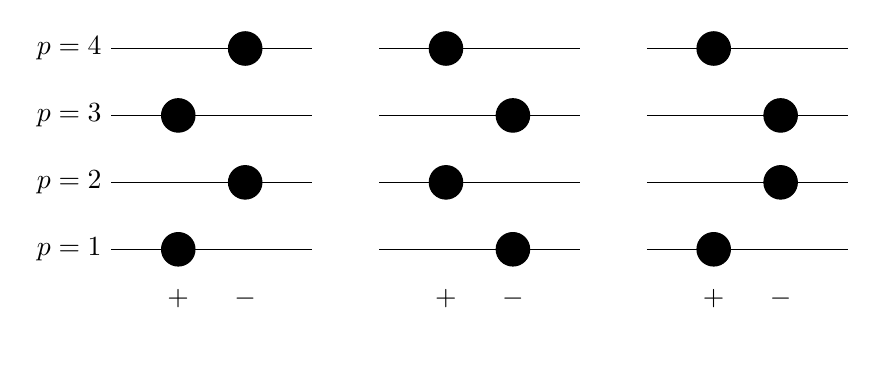
\begin{tikzpicture}[scale=0.85]
    \begin{scope}
      \foreach \i in {1,...,4}
      {
        \draw (-1,\i-1) node[anchor=east] {$p = \i$} --(2,\i-1);
      }
      \filldraw (0,0) node[anchor=north,inner sep=.5cm] {$+$} ; 
      \filldraw (1,0) node[anchor=north,inner sep=.5cm] {$-$} ;
      \filldraw (0,0) circle (0.25cm); 
      \filldraw (0,2) circle (0.25cm); 
      \filldraw (1,1) circle (0.25cm); 
      \filldraw (1,3) circle (0.25cm);
    \end{scope}
    \begin{scope}[xshift=4cm]
      \foreach \i in {1,...,4}
      {
        \draw (-1,\i-1) --(2,\i-1);
      }
      \filldraw (0,0) node[anchor=north,inner sep=.5cm] {$+$} ; 
      \filldraw (1,0) node[anchor=north,inner sep=.5cm] {$-$} ;
      \filldraw (0,1) circle (0.25cm); 
      \filldraw (0,3) circle (0.25cm); 
      \filldraw (1,0) circle (0.25cm); 
      \filldraw (1,2) circle (0.25cm);
    \end{scope}
    \begin{scope}[xshift=8cm]
      \foreach \i in {1,...,4}
      {
        \draw (-1,\i-1) --(2,\i-1);
      }
      \filldraw (0,0) node[anchor=north,inner sep=.5cm] {$+$} ; 
      \filldraw (1,0) node[anchor=north,inner sep=.5cm] {$-$} ;
      \filldraw (0,0) circle (0.25cm); 
      \filldraw (0,3) circle (0.25cm); 
      \filldraw (1,1) circle (0.25cm); 
      \filldraw (1,2) circle (0.25cm);
    \end{scope}
  \end{tikzpicture}
  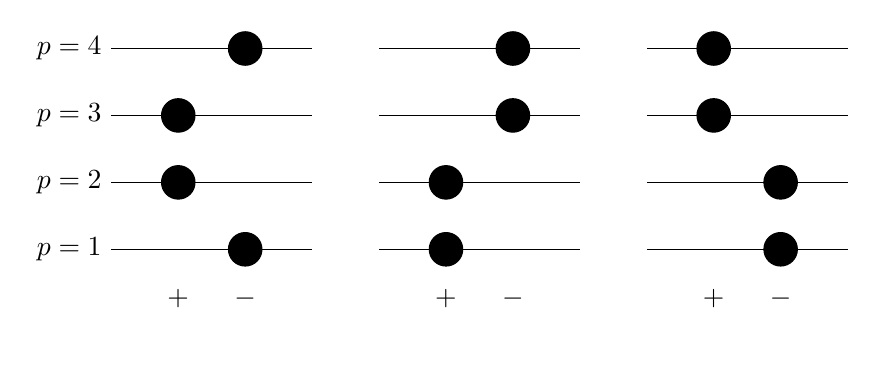
\begin{tikzpicture}[scale=0.85]
      \begin{scope}[xshift=0cm]
      \foreach \i in {1,...,4}
      {
        \draw (-1,\i-1) node[anchor=east] {$p = \i$} --(2,\i-1);
      }
      \filldraw (0,0) node[anchor=north,inner sep=.5cm] {$+$} ; 
      \filldraw (1,0) node[anchor=north,inner sep=.5cm] {$-$} ;
      \filldraw (1,0) circle (0.25cm); 
      \filldraw (1,3) circle (0.25cm); 
      \filldraw (0,1) circle (0.25cm); 
      \filldraw (0,2) circle (0.25cm);
    \end{scope}
    \begin{scope}[xshift=4cm]
      \foreach \i in {1,...,4}
      {
        \draw (-1,\i-1) --(2,\i-1);
      }
      \filldraw (0,0) node[anchor=north,inner sep=.5cm] {$+$} ; 
      \filldraw (1,0) node[anchor=north,inner sep=.5cm] {$-$} ;
      \filldraw (0,0) circle (0.25cm); 
      \filldraw (0,1) circle (0.25cm); 
      \filldraw (1,2) circle (0.25cm); 
      \filldraw (1,3) circle (0.25cm);
    \end{scope}
    \begin{scope}[xshift=8cm]
      \foreach \i in {1,...,4}
      {
        \draw (-1,\i-1) --(2,\i-1);
      }
      \filldraw (0,0) node[anchor=north,inner sep=.5cm] {$+$} ; 
      \filldraw (1,0) node[anchor=north,inner sep=.5cm] {$-$} ;
      \filldraw (1,0) circle (0.25cm); 
      \filldraw (1,1) circle (0.25cm); 
      \filldraw (0,2) circle (0.25cm); 
      \filldraw (0,3) circle (0.25cm);
    \end{scope}
  \end{tikzpicture}
\end{center}
\caption{All the basis states in the subspace of the Hilbert space with $S_z=0$, $P=0$, $N=4$, and $M=4$. \label{fig:10}}
\end{figure}
Assuming we are restricted to the $N=4$ case, we have the possible basis set shown in \fig{10}.


\begin{exframe}
\begin{itemize}
  \item[h)] Show that you can rewrite the Hamiltonian (with $\xi=1$) as 
  \begin{align}
  \hat H = \sum_p (p-1)\hat n_p - \frac{1}{2}g \left( \sum_p \hat P^\dagger_p \right) \left( \sum_q \hat P_q  \right).
  \end{align}
\end{itemize}
\end{exframe}
Inserting the definitions $\epsilon_p$ and $\hat V$ with $\hat P_p$ and $\hat P^\dagger_q$ we find
\begin{align}
\hat H &= \sum_\ps \epsilon_p c_\ps^\dagger c_\ps - \frac{1}{2}g \sum_{pq} \cppd \cpmd \cqm \cqp \nn\\
%
&= \sum_p (p-1) \left(\cppd \cpp + \cpmd \cpm \right) - \frac{1}{2}g \left(\sum_p\cppd \cpmd \right) \left( \sum_q \cqm \cqp \right) \nn\\
%
&= \sum_p (p-1) \hat n_p - \frac{1}{2}g \left(\sum_p\hat P_p^\dagger\right) \left( \sum_q \hat P_q\right).
\end{align}

\newpage
\subsection*{Exercise 2}
\begin{exframe}
\begin{itemize}
  \item[a)] Show that $\sum_s \hat P_s |p\bar p q \bar q\rangle = |p\bar p\rangle + |q \bar q\rangle$. Next, compute the closed form expression for all the matrix elements $\left\langle p'\bar p' q' \bar q' \right|\hat H \left|p\bar p q \bar q \right\rangle$.
\end{itemize}
\end{exframe}
From now on, states labeled by capital letters denote pair states, i.e. $|IJ\rangle = |i\bar i j\bar j\rangle$, with $i$ and $j$ being single particle orbital indices. We use the numbering shown in \fig{1}.

Operating on a state of two pairs with $\sum_p \hat P$ yields
\begin{align}
\sum_r \hat P_r |p\bar p q\bar q\rangle &= \hat P_p |p\bar p q\bar q\rangle + \hat P_q |p\bar p q\bar q\rangle \nn\\
%
&= |p\bar p \rangle + |q\bar q\rangle,
\end{align}
where all the terms in the sum vanish, except for when the $r$-pair is in the Slater.

Let us now compute the matrix elements of the total Hamiltonian. We find that
\begin{align}
\left\langle p\bar p q\bar q \right| \hat H \left| r \bar r s \bar s \right\rangle &= \left\langle PQ \left| \hat H_0 + \hat V  \right| RS \right\rangle \nn\\
%
&= \left\langle PQ \left| \sum_j (j-1) \hat n_j \right| RS \right\rangle -\left\langle PQ \left| \frac{1}{2}g \left(\sum_i\hat P_i^\dagger\right) \left( \sum_j \hat P_j\right)  \right| RS \right\rangle,
\end{align}
where 
\begin{align}
\left\langle PQ \left| \sum_j (j-1) \hat n_j \right| RS \right\rangle &= \left\langle p \bar p q \bar q \left| \sum_j (j-1) \hat n_j \right| r\bar r s\bar s\right\rangle \nn\\
% 
&= \left\langle p \bar p q \bar q \left| \big[ (r-1)\hat n_r + (s-1)\hat n_s \big] \right| r\bar r s\bar s\right\rangle \nn\\
%
&= \left\langle p \bar p q \bar q \left| \big[ (r-1)\big( c_{r+}^\dagger c_{r+} + c_{r-}^\dagger c_{r-} \big) + (s-1)\big( c_{s+}^\dagger c_{s+} + c_{s-}^\dagger c_{s-} \big) \big] \right| r\bar r s\bar s\right\rangle \nn\\
% 
&= \left\langle p \bar p q \bar q \left| \big[ 2(r-1) + 2(s-1) \big] \right| r\bar r s\bar s\right\rangle \nn\\
%
&= 2(r-1) \langle p \bar p q \bar q | r\bar r s\bar s\rangle + 2(s-1) \langle p \bar p q \bar q | r\bar r s\bar s\rangle \nn\\
%
&= 2(r-1) \delta_{pr}\delta_{qs} + 2(s-1) \delta_{pr}\delta_{qs} \nn\\
%
&= 2\delta_{pr}\delta_{qs} \big[r+s-2\big],
\end{align}
and 
\begin{align}
\left\langle PQ \left| \frac{1}{2}g \left(\sum_i\hat P_i^\dagger\right) \left( \sum_j \hat P_j\right)  \right| RS \right\rangle &= \frac{1}{2}g\left\langle PQ \left|  \left(\sum_i\hat P_i^\dagger\right) \left(\hat P_r + \hat P_s\right)  \right| RS \right\rangle \nn\\
%
&= \frac{1}{2}g\left\langle PQ \left|  \left(\sum_i\hat P_i^\dagger\right)\right|  \Big[\big |R\big\rangle + \big |S\big\rangle  \Big] \right) \nn\\
%
&= \frac{1}{2}g \left\langle \left(\sum_i\hat P_i^\dagger\right)^\dagger PQ \Bigg|  \Big[\big |R\big\rangle + \big |S\big\rangle  \Big] \right) \nn\\
%
&= \frac{1}{2}g \left\langle \left(\sum_i\hat P_i\right) PQ \Bigg|  \Big[\big |R\big\rangle + \big |S\big\rangle  \Big] \right) \nn\\
%
&= \frac{1}{2}g \left\langle \left(\hat P_p + \hat P_q\right) PQ \Big|  \Big[\big |R\big\rangle + \big |S\big\rangle  \Big] \right) \nn\\
%
&= \frac{1}{2}g  \Big[\big\langle P\big| + \big \langle Q\big|  \Big] \Big|  \Big[\big |R\big\rangle + \big |S\big\rangle  \Big] \nn
\end{align}
\begin{align}
&= \frac{1}{2}g \Big(   \left\langle P\big| R\right\rangle + \left\langle P\big| S\right\rangle  + \left\langle Q\big| R\right\rangle  + \left\langle Q\big| S\right\rangle  \Big) \nn\\
%
&= \frac{1}{2}g \Big(   \left\langle p\bar p | r \bar r\right\rangle + \left\langle p \bar p| s\bar s\right\rangle  + \left\langle q \bar q| r \bar r\right\rangle  + \left\langle q\bar q|s \bar s\right\rangle  \Big) \nn\\
%
&= \frac{1}{2}g \Big( \delta_{pr} + \delta_{ps} + \delta_{qr} + \delta_{qs}\Big).
\end{align}
Combining $\langle \Phi | \hat H_0 | \Phi \rangle$ and $\langle \Phi | \hat V | \Phi \rangle$ we find the matrix elements of the total Hamiltonian as 
\begin{align}
\left\langle p\bar p q\bar q \right| \hat H \left| r \bar r s \bar s \right\rangle &= 2\delta_{pr}\delta_{qs} \big[r+s-2\big] - \frac{1}{2}g \Big( \delta_{pr} + \delta_{ps} + \delta_{qr} + \delta_{qs}\Big). \label{eq:5}
\end{align}

\begin{exframe}
\begin{itemize}
  \item[b)] We now set $\xi=1$, and consider $g\in [-1,1]$. Using your favorite compting environment, diagonalize the Hamiltonian matrix numerically. Plot the eigenvalues $E_k=E_k(g)$ as function of $g$ in a single figure. Highlight the ground-state energy. Do you observe any degeneracies?
\end{itemize}
\end{exframe}
\begin{figure}
\centering
\includegraphics[width=12cm]{FCI_E.pdf}
\caption{The energies found from full configuration-interaction as functions of the two-particle potential strength, $g$. We note that energies three and four coincide, i.e. this is a degenerate energy level. \label{fig:2}}
\end{figure}
\begin{figure}
\centering
\includegraphics[width=12cm]{FCI_f.pdf}
\caption{The probability of finding the system in the unperturbed ground state, $f_\text{FCI}(g)=|\langle 1|\Psi(g)\rangle|^2$\label{fig:3}}
\end{figure}
The relevant\footnote{Some parts are ommitted for clarity (setting of variables, plotting, etc.).} parts of the {\sc Matlab} code for diagonalizing the full configuration-interaction matrix is shown in the appendix. The entire code is available at \url{https://github.com/mortele/FYS-KJM4480/tree/master/Project2}.

Using the capital letter notation for the states with the numbering shown in \fig{1}, the FCI matrix looks like
\begin{align}
H_\text{FCI} = \left[ \langle I |\hat H|J\rangle \right]_{IJ} =  \bmat{cccccc}{\langle 1|\hat H |1\rangle & \langle 1|\hat H |2\rangle & \langle 1|\hat H |3\rangle & \langle 1|\hat H |4\rangle & \langle 1|\hat H |5\rangle & \langle 1|\hat H |6\rangle \\
\langle 2|\hat H |1\rangle & \langle 2|\hat H |2\rangle & \langle 2|\hat H |3\rangle & \langle 2|\hat H |4\rangle & \langle 2|\hat H |5\rangle & \langle 2|\hat H |6\rangle \\
\langle 3|\hat H |1\rangle & \langle 3|\hat H |2\rangle & \langle 3|\hat H |3\rangle & \langle 3|\hat H |4\rangle & \langle 3|\hat H |5\rangle & \langle 3|\hat H |6\rangle \\
\langle 4|\hat H |1\rangle & \langle 4|\hat H |2\rangle & \langle 4|\hat H |3\rangle & \langle 4|\hat H |4\rangle & \langle 4|\hat H |5\rangle & \langle 4|\hat H |6\rangle \\
\langle 5|\hat H |1\rangle & \langle 5|\hat H |2\rangle & \langle 5|\hat H |3\rangle & \langle 5|\hat H |4\rangle & \langle 5|\hat H |5\rangle & \langle 5|\hat H |6\rangle \\
\langle 6|\hat H |1\rangle & \langle 6|\hat H |2\rangle & \langle 6|\hat H |3\rangle & \langle 6|\hat H |4\rangle & \langle 6|\hat H |5\rangle & \langle 6|\hat H |6\rangle}.
\end{align}
We note that $H_\text{FCI}\in \R^{6\times6}$. The energies as functions of the varying $g$ are shown in \fig{2}. We note the degeneracies in energy levels three and four. The ground state energy is highlighted (bold line). Since $\hat V$ has an overall minus sign, a positive $g$ coefficient means pairing is energetically favorable. We can see this from the negative slopes in \fig{2}: As $g$ increases, all the states decrease in energy. The opposite is true for negative $g$, when pairing is energetically un-favorable.

The probability of finding the system in the unperturbed ground state as a function of $g$ is shown in \fig{3}. We note that for $g=0$, we are in the unperturbed system and $f_\text{FCI}=1$. For positive $g$, when pairing becomes favorable, the ground state (of the full problem) shifts relatively rapidly away from the unperturbed ground state. For negative $g$, when pairing yields higher energies, this shift is less pronounced as expected. 

\begin{exframe}
\begin{itemize}
  \item[c)] We now turn to CISD approximation, using $|\Phi\rangle = |1\rangle$ as the reference. Explain why the sinly excited determinants will not contribute to the exact eigenfunction, i.e. that CISD is the same as CID. 

  Show that the doubly excited determinants can be written 
  \begin{align}
  \left|\Phi_{i\bar i}^{a\bar a}\right\rangle\equiv \hat P_a^\dagger P_i |\Phi\rangle, \ \ \ i=1,2, \ \ a=3,4.
  \end{align}
  What is the dimension of the CID space? How many basis functions from the FCI space do you miss?

  Find the CID Hamiltonian matrix. Diagonalize this matrix numerically for $g\in [-1,1]$ and plot the \emph{ground-state} eigenvalue as a function of $g$. Plot also the ground-state probaility. Compare with FCI and discuss.
\end{itemize}
\end{exframe}
\begin{figure}
\centering
\includegraphics[width=12cm]{CID_E.pdf}
\caption{ The energies found from configuration-interaction doubles as functions of the two-particle potential strength, $g$. \label{fig:4}}
\end{figure}
\begin{figure}
\centering
\includegraphics[width=12cm]{CID_f.pdf}
\caption{The probability of finding the system in the unperturbed ground state, $f_\text{CID}(g)=|\langle 1|\Psi(g)\rangle|^2$\label{fig:5}}
\end{figure}
The singly excited states, $|\Phi_i^a\rangle = c^\dagger_a c_i |\Phi\rangle$, have one of the pairs in $|\Phi\rangle$ broken. In other words, $\hat P|\Phi_i^a\rangle = 1|\Phi_i^a\rangle$, as only a single pair is left. But we know that $[\hat H, \hat P]=0$ and so $\hat H$ preserves the number of pairs. This means 
\begin{align}
\langle \Phi | \hat H | \Phi_i^a\rangle &= \big\langle \Phi \big| \left( \sum_j \alpha_j \big|\Psi_j\big\rangle \right) = 0,
\end{align}
where $\alpha_j\in\R$ and $\Psi_j$ are some states with $P=1$. We note that $\langle \Phi | \Psi_j\rangle=0$ for any such state. This means in effect that singly excited states will not couple to the reference, or the doubly excited states and as such will not contribute to the ground state energy. 

For CISD, the Hamiltonian matrix will have structure as follows:
\begin{align}
H_\text{CISD} = \bmat{ccc}{\\ \bmat{ccc}{& & \\ & \big\langle I \big| \hat H\big| J \big\rangle & \\ & & } & & \bmat{ccc}{& & \\ & \big\langle I \big| \hat H\big| J_{i\bar i}^{a\bar a} \big\rangle & \\ & & } \\
& \bmat{ccc}{& & \\ & \big\langle I_i^a \big| \hat H\big| J_j^b \big\rangle & \\ & & } & \\
\bmat{ccc}{& & \\ & \big\langle I_{i\bar i}^{a\bar a} \big| \hat H\big| J \big\rangle & \\ & & } & & \bmat{ccc}{& & \\ & \big\langle I_{i\bar i}^{a \bar a} \big| \hat H\big| J_{j\bar j}^{b\bar b} \big\rangle & \\ & & } \\ &},
\end{align} 
where ommitted entries are all zero. We see clearly from this structure that just removing the singles entries will not affect the diagonalized states and energies for CID. 

The doubly excited states, written in terms of creation operators relative to the true vacuum, are defined as $|\Phi_{ij}^{ab}\rangle=c^\dagger_a c^\dagger_b c_i c_j |\Phi\rangle$. Restricted to the subspace of $P=2$, $S_z=0$, the only allowed excitations are two excitations from level $p$ under the Fermi level (i.e. $p\le 2$) up to two excitations to level $a$ over the Fermi level (i.e. $a\ge 3$). Obviously, either excited orbital will need to have different spin-projection in order to preserve $S_z=0$. This means $|\Phi_{ij}^{ab}\rangle=c^\dagger_a c^\dagger_{\bar a} c_i c_{\bar i} |\Phi\rangle = \hat P^\dagger_a \hat P_i |\Phi\rangle$.

The only state which can \emph{not} be reached by only exciting one pair from the reference state is the state denoted number six in \fig{1}. However, all of the other states are contained in the CID space, meaning this subspace has dimension five. 

The relevant parts of the {\sc Matlab} code for diagonalizing the configuration-interaction doubles matrix is shown in the appendix. The entire code is once again available at \url{https://github.com/mortele/FYS-KJM4480/tree/master/Project2}. 

The resulting energies and ground state probabilities are shown in Figs. (\ref{fig:4}) and (\ref{fig:5}). We note that the degeneracy from FCI is broken when the sixth state is removed. We also note that this highly excited sixth state is not very relevant for the ground (unperturbed) ground state probability, meaning removing it does not change the probability very much (after diagonlizing, the coefficient $(H_\text{FCI})_{1,6}\propto0.05$).


\begin{exframe}
\begin{itemize}
  \item[d)] Next up is Rayleigh-Schrödinger pertubation theory. Write down the expression for third-order pertubation theory for the ground-state energy for this model. Which matrix elements of $\hat H$ are needed?
\end{itemize}
\end{exframe}
Using the same notation as before ($|\Phi\rangle = |12\rangle$), and defining the projection operator 
\begin{align}
\hat R = \sum_{j\not=k} \frac{1}{\varepsilon_k-\varepsilon_j}|\phi_j\rangle \langle \phi_j| \equiv \sum_{j\not=k} \gamma_j |\phi_j\rangle \langle \phi_j|,
\end{align}
with $\gamma_{ij} \equiv 1/(\varepsilon_{12}-\varepsilon_{ij})$, we can write the first, second, and third corrections to the $k=1$ energy according to RSPT3 as
\begin{align}
E^{(0)}_1 &= \langle \phi_1 |\hat H_0 |\phi_1\rangle, \\
%
E^{(1)}_1 &= \langle \phi_1 |\hat V |\phi_1\rangle, \\
%
E^{(2)}_1 &= \langle \phi_1 |\hat V \hat R \hat V |\phi_1\rangle, \ \ \text{ and }\\
%
E^{(3)}_1 &= \langle \phi_1 |\hat V \hat R \hat V \hat R \hat V |\phi_1\rangle - E^{(1)}\langle \phi_1 |\hat V \hat R^2 \hat V |\phi_1\rangle.
\end{align}
From now on, we will ommit the subscript 1, and use $|\phi_1\rangle = |\Phi\rangle = |12\rangle$. 

Computing $E^{(0)}=\langle 12 | \hat H_0 | 12\rangle=2(1-1)\langle12|12\rangle+2(2-1)\langle12|12\rangle=2$ is easy, and $E^{(1)}=-g$ can be seen from \eq{5}. Moving on, we can write out the expression for $E^{(2)}$ as
\begin{align}
E^{(2)} &= \langle \phi_1 |\hat V \hat R \hat V |\phi_1\rangle \nn\\
%
&= -\frac{1}{2}g\left\langle 12 \Bigg| \hat V \hat R \left(\sum_p \hat P^\dagger_p \right)\left( \sum_q \hat P_q \right) \Bigg| 12\right\rangle \nn\\
%
&= -\frac{1}{2}g\left\langle 12 \Bigg| \hat V \hat R \left(\sum_p \hat P^\dagger_p \right) \left[  \hat P_1 + \hat P_2  \right]  \Bigg| 12\right\rangle  \nn\\
%
&= -\frac{1}{2}g\left\langle 12 \Bigg| \hat V \hat R \left(\sum_p \hat P^\dagger_p \right)   \right| \Big[ \big|1\big\rangle + \big|2\big\rangle\Big] \nn\\
%
&= -\frac{1}{2}g\left\langle 12 \Bigg| \hat V \hat R \left[  \hat P^\dagger_1 + \hat P^\dagger_2 + P^\dagger_3 + P^\dagger_4  \right]   \right| \Big[ \big|1\big\rangle + \big|2\big\rangle\Big] \nn\\
%
&= -\frac{1}{2}g\left\langle 12 \Big| \hat V \hat R \right| \Big[ \big|12\big\rangle + \big|12\big\rangle + \big|13\big\rangle + \big|14\big\rangle + \big|23\big\rangle + \big|24\big\rangle\Big] \nn\\
%
&= -\frac{1}{2}g\left\langle 12 \Big| \hat V \sum_{j\not=1}\gamma_j |\phi_j\rangle\langle \phi_j| \right| \Big[ 2\big|12\big\rangle + \big|13\big\rangle + \big|14\big\rangle + \big|23\big\rangle + \big|24\big\rangle\Big] \nn\\
%
&= -\frac{1}{2}g\Big\langle 12 \Big| \hat V \sum_{j\not=1}\gamma_j |\phi_j\rangle\langle \phi_j|  \Big[ 2\big|12\big\rangle + \big|13\big\rangle + \big|14\big\rangle + \big|23\big\rangle + \big|24\big\rangle\Big] \nn\\
%
&= -\frac{1}{2}g\Big\langle 12 \Big| \hat V \Big(\gamma_{13} |13\rangle\langle 13| + \gamma_{14} |14\rangle\langle 14| + \gamma_{23} |23\rangle\langle 23| + \gamma_{24} |24\rangle\langle 24| + \gamma_{34} |34\rangle\langle 34| \Big) \nn\\ 
& \ \ \ \ \ \ \ \ \ \ \ \ \ \ \ \ \ \ \ \ \ \ \ \ \ \ \ \ \ \ \ \ \ \ \ \ \ \ \ \ \ \ \ \ \ \ \ \ \ \ \ \ \ \ \ \ \ \ \ \ \ \ \ \ \ \ \ \ \ \ \ \ \ \ \ \ \ \ \Big[ 2\big|12\big\rangle + \big|13\big\rangle + \big|14\big\rangle + \big|23\big\rangle + \big|24\big\rangle\Big] \nn\\
%
&= -\frac{1}{2}g\Big\langle 12 \Big| \hat V \Big[ \gamma_{13}\big|13\big\rangle + \gamma_{14}\big|14\big\rangle + \gamma_{23}\big|23\big\rangle + \gamma_{24}\big|24\big\rangle\Big] \nn\\
%
&= -\frac{1}{2}g\Big( \gamma_{13}\big\langle12\big|\hat V\big|13\big\rangle + \gamma_{14}\big\langle12\big|\hat V\big|14\big\rangle + \gamma_{23}\big\langle12\big|\hat V\big|23\big\rangle + \gamma_{24}\big\langle12\big|\hat V\big|24\big\rangle\Big).
\end{align}
Secondly, we move on to consider $E^{(3)}$, which we split in two. For simplicity, let us first compute $\hat R^2$ as
\begin{align}
\hat R^2 &= \hat R \hat R = \Big( \gamma_{13} |13\rangle\langle 13| + \gamma_{14} |14\rangle\langle 14| + \gamma_{23} |23\rangle\langle 23| + \gamma_{24} |24\rangle\langle 24| + \gamma_{34} |34\rangle\langle 34|  \Big) \nn\\
& \ \ \ \ \ \ \ \ \ \ \ \ \ \ \ \ \ \ \ \ \ \ \ \ \ \ \ \ \Big( \gamma_{13} |13\rangle\langle 13| + \gamma_{14} |14\rangle\langle 14| + \gamma_{23} |23\rangle\langle 23| + \gamma_{24} |24\rangle\langle 24| + \gamma_{34} |34\rangle\langle 34|  \Big) \nn\\
%
&= \Big( \gamma_{13}^2 |13\rangle\langle 13|13\rangle\langle 13| + \gamma_{14}^2 |14\rangle\langle 14|14\rangle\langle 14| + \gamma_{23}^2 |23\rangle\langle 23|23\rangle\langle 23| \nn\\
& \ \ \ \ \ \ \ \ \ \ \ \ \ \ \ \ \ \ \ \ \  \ \ \ \ \ \ \ \ \ \ \ \ \ \ +  \gamma_{24}^2 |24\rangle\langle 24|24\rangle\langle 24| + \gamma_{34}^2 |34\rangle\langle 34|34\rangle\langle 34|  \Big) \nn\\
%
&= \Big( \gamma_{13}^2 |13\rangle\langle 13| + \gamma_{14}^2 |14\rangle\langle 14| + \gamma_{23}^2 |23\rangle\langle 23| + \gamma_{24}^2 |24\rangle\langle 24| + \gamma_{34}^2 |34\rangle\langle 34|  \Big),
\end{align}
where every single cross term vanishes due to the orthogonality of the states. With this in mind, let us consider the second term of $E^{(3)}$. We note that we already know the action of $\hat V$ on $|12\rangle$ from the calculation of $E^{(2)}$, so we start from there
\begin{align}
E^{(3)}_\text{second term} &= E^{(1)}\langle \phi_1 |\hat V \hat R^2 \hat V |\phi_1\rangle \nn\\
%
&= \frac{1}{2}g^2 \Big\langle 12 \Big| \hat V \hat R^2 \Bigg[ 2\Big|12\Big\rangle +  \Big|13\Big\rangle + \Big|14\Big\rangle + \Big|23\Big\rangle + \Big|24\Big\rangle\Bigg] \nn\\
%
&= \frac{1}{2}g^2 \Big\langle 12 \Big| \hat V \Bigg[  \gamma_{13}^2\Big|13\Big\rangle + \gamma_{14}^2\Big|14\Big\rangle + \gamma_{23}^2\Big|23\Big\rangle + \gamma_{24}^2\Big|24\Big\rangle\Bigg] \nn\\
%
&= \frac{1}{2}g^2 \Big(  \gamma_{13}^2\big\langle12\big|\hat V\big|13\big\rangle + \gamma_{14}^2\big\langle12\big|\hat V\big|14\big\rangle + \gamma_{23}^2\big\langle12\big|\hat V\big|23\big\rangle + \gamma_{24}^2\big\langle12\big|\hat V\big|24\big\rangle \Big).
\end{align}
Lastly, we consider the first term of $E^{(3)}$ and find
\begin{align}
E^{(3)}_\text{first term} &= \langle \phi_1 |\hat V \hat R \hat V \hat R \hat V |\phi_1\rangle \nn\\
%
&= -\frac{1}{2}g \big\langle 12 \big| \hat V \hat R \hat V \Big[ \gamma_{13}\big| 13\big\rangle + \gamma_{14}\big| 14\big\rangle +\gamma_{23} \big| 23\big\rangle + \gamma_{24} \big| 24\big\rangle \Big] \nn\\
%
&= \frac{1}{4}g^2 \big\langle 12 \big| \hat V \hat R \bigg[ \gamma_{13}\Big(2\big| 13\big\rangle + \big| 14\big\rangle + \big| 23\big\rangle + \big| 34\big\rangle \Big) \nn\\
& \ \ \ \ \ \ \ \ \ \ \ \ \ \ \ \ \ + \gamma_{14}\Big(2\big| 14\big\rangle + \big| 13\big\rangle + \big| 24\big\rangle + \big| 34\big\rangle \Big) \nn\\ 
& \ \ \ \ \ \ \ \ \ \ \ \ \ \ \ \ \ \ \ \ \ \ + \gamma_{23}\Big(2\big| 23\big\rangle + \big| 24\big\rangle + \big| 13\big\rangle + \big| 34\big\rangle \Big) \nn\\ 
& \ \ \ \ \ \ \ \ \ \ \ \ \ \ \ \ \ \ \ \ \ \ \ \ \ \ \ + \gamma_{24}\Big(2\big| 24\big\rangle + \big| 14\big\rangle + \big| 23\big\rangle + \big| 34\big\rangle \Big)\bigg] \nn\\ 
%
&= \frac{1}{4}g^2 \big\langle 12 \big| \hat V \bigg[ \gamma_{13}^2\Big(2\big| 13\big\rangle + \big| 14\big\rangle + \big| 23\big\rangle + \big| 34\big\rangle \Big) \nn\\
& \ \ \ \ \ \ \ \ \ \ \ \ \ \ \ \ \ + \gamma_{14}^2\Big(2\big| 14\big\rangle + \big| 13\big\rangle + \big| 24\big\rangle + \big| 34\big\rangle \Big) \nn\\ 
& \ \ \ \ \ \ \ \ \ \ \ \ \ \ \ \ \ \ \ \ \ \ + \gamma_{23}^2\Big(2\big| 23\big\rangle + \big| 24\big\rangle + \big| 13\big\rangle + \big| 34\big\rangle \Big) \nn\\ 
& \ \ \ \ \ \ \ \ \ \ \ \ \ \ \ \ \ \ \ \ \ \ \ \ \ \ \ + \gamma_{24}^2\Big(2\big| 24\big\rangle + \big| 14\big\rangle + \big| 23\big\rangle + \big| 34\big\rangle \Big)\bigg] \nn\\ 
%
&= \frac{1}{4}g^2 \bigg[ \gamma_{13}^2\Big(2\big\langle 12 \big| \hat V \big| 13\big\rangle + \big\langle 12 \big| \hat V \big| 14\big\rangle + \big\langle 12 \big| \hat V \big| 23\big\rangle + \big\langle 12 \big| \hat V \big| 34\big\rangle \Big) \nn\\
& \ \ \ \ \ \ \ \ \ \ \ \ \ \ \ \ \ + \gamma_{14}^2\Big(2\big\langle 12 \big| \hat V \big| 14\big\rangle + \big\langle 12 \big| \hat V \big| 13\big\rangle + \big\langle 12 \big| \hat V \big| 24\big\rangle + \big\langle 12 \big| \hat V \big| 34\big\rangle \Big) \nn\\ 
& \ \ \ \ \ \ \ \ \ \ \ \ \ \ \ \ \ \ \ \ \ \ + \gamma_{23}^2\Big(2\big\langle 12 \big| \hat V \big| 23\big\rangle + \big\langle 12 \big| \hat V \big| 24\big\rangle + \big\langle 12 \big| \hat V \big| 13\big\rangle + \big\langle 12 \big| \hat V \big| 34\big\rangle \Big) \nn\\ 
& \ \ \ \ \ \ \ \ \ \ \ \ \ \ \ \ \ \ \ \ \ \ \ \ \ \ \ + \gamma_{24}^2\Big(2\big\langle 12 \big| \hat V \big| 24\big\rangle + \big\langle 12 \big| \hat V \big| 14\big\rangle + \big\langle 12 \big| \hat V \big| 23\big\rangle + \big\langle 12 \big| \hat V \big| 34\big\rangle \Big) \bigg].
\end{align}

We note that $\langle PQ|\hat V | RS\rangle $ are simply elements of the FCI Hamiltonian (because the offdiagonal elements of $\hat H$ have vanishing $\hat H_0$ contributions). This means we need the first row of elements from the FCI matrix.

\begin{exframe}
\begin{itemize}
  \item[e)] Compute the ground-state energy to third order in Rayleigh-Schrödinger pertubation theory, i.e. compute the third order expansion in $g$, 
  \begin{align}
  E_\text{RSPT3}(g) &= E^{(0)} + gE^{(1)} + g^2E^{(2)} + g^3E^{(3)}.
  \end{align}
\end{itemize}
\end{exframe}
\begin{figure}
\centering
\includegraphics[width=12cm]{RS_E.pdf}
\caption{Ground state energy correction computed by third order Rayleigh-Schrödinger pertubation theory. First and second order is also shown. \label{fig:6}}
\end{figure}
The relevant parts of the {\sc Matlab} code for computing the third order expansion in $g$ is shown in the appendix. The entire code is available at \url{https://github.com/mortele/FYS-KJM4480/tree/master/Project2}. The resulting energy is shown for first, second, and third order expansion in \fig{6}.



\subsection*{Exercise 3}
The last task is a coupled-cluster treatment, with doubles only, CCD. We will use a doubles operator on the form 
\begin{align}
\hat T = \sum_{ia} t^a_i b_{a+}^\dagger b_{i+}^\dagger b_{a-}^\dagger b_{i-}^\dagger = \sum_{ia} t^a_i \hat P_a^\dagger \hat P_i.
\end{align}
\begin{exframe}
\begin{itemize}
  \item[a)] Write down the general CCD wavefunction in terms of $\hat T$ and $|\Phi\rangle$. Explain why the exponential truncates after second-order terms for our model.
\end{itemize}
\end{exframe}
The general CCD wavefunction can be written as 
\begin{align}
|\Phi_\text{CCD}\rangle &= \left(1 + \hat T + \frac{1}{2!}\hat T^2 + \frac{1}{3!}\hat T^3 + \dots \right) |\Phi\rangle. \label{eq:6}
\end{align}
If we consider the action of $\hat T$ on $|\Phi\rangle$ we find
\begin{align}
\hat T |\Phi\rangle &= \sum_{ia} t^a_i \hat P_a^\dagger \hat P_i |12\rangle \nn\\
%
&= \sum_{a} \hat P_a^\dagger \big[ t^a_2|1\rangle +  t^a_1|2\rangle \big] \nn\\
%
&=  t^3_2|13\rangle + t^4_2|14\rangle + t^3_1|23\rangle + t^4_1|24\rangle.
\end{align}
Applying $\hat T$ a second time, we find
\begin{align}
\hat T^2 |\Phi\rangle &= \hat T\Big[ t^3_2|13\rangle + t^4_2|14\rangle + t^3_1|23\rangle + t^4_1|24\rangle \Big] \nn\\
%
&= \sum_{ia} t^a_i \hat P^\dagger_a \hat P_i  \Big[ t^3_2|13\rangle + t^4_2|14\rangle + t^3_1|23\rangle + t^4_1|24\rangle \Big] \nn\\
%
&= \sum_{a} \hat P^\dagger_a \Big[ t_1^at^3_2|3\rangle + t_1^at^4_2|4\rangle + t^a_2t^3_1|3\rangle + t_2^at^4_1|4\rangle \Big] \nn\\
%
&= t_1^4t^3_2|34\rangle + t_1^3t^4_2|34\rangle + t^4_2t^3_1|34\rangle + t_2^3t^4_1|34\rangle \nn\\
%
&= \Big[ t_1^4t^3_2 + t_1^3t^4_2 + t^4_2t^3_1 + t_2^3t^4_1 \Big] |34\rangle, \label{eq:9}
\end{align}
from which we note that $\hat T^3 |\Phi\rangle=0$ since there are no orbitals in the state left \emph{under} the Fermi level and so applying $\sum_i \hat P_i$ yields zero. This obviously means the expansion in \eq{6} truncates after two terms, which gives the CCD wavefunction as
\begin{align}
|\Phi_\text{CCD}\rangle &= \left(1 + \hat T + \frac{1}{2}\hat T^2 \right) |\Phi\rangle. \label{eq:7}
\end{align}

\begin{exframe}
\begin{itemize}
  \item[b)] In a similar manner, write down the general CID wavefunction in intermediate normalization, $\langle \Phi | \Psi_\text{CID}\rangle=1$. Compare with the CCD wavefunction.
\end{itemize}
\end{exframe}
The general CI wavefunction can be written as 
\begin{align}
|\Psi_\text{CI}\rangle &= c_0 |\Phi\rangle + \sum_i \sum_a c_i^a |\Phi^a_i\rangle + \sum_{ij} \sum_{ab} c_{ij}^{ab} |\Phi^{ab}_{ij}\rangle + \sum_{ijk} \sum_{abc} c_{ijk}^{abc} |\Phi^{abc}_{ijk}\rangle + \dots,
\end{align}
with the constants $c_{ijk\dots}^{abc\dots} = \langle \Phi_{ijk\dots}^{abc\dots} |\Psi_\text{CI}\rangle$. Specifically, the CID wavefunction can be written as 
\begin{align}
|\Psi_\text{CID}\rangle &= c_0 |\Phi\rangle + \sum_{ij} \sum_{ab} c_{ij}^{ab} |\Phi^{ab}_{ij}\rangle. \label{eq:8}
\end{align}
Comparing now Eqs. (\ref{eq:6}) and (\ref{eq:8}), we see striking similarities but the CID wavefunction is lacking the quadruple excitations in $\hat T^2$.

\begin{exframe}
\begin{itemize}
  \item[c)] Explain that the CCD energy can be written 
  \begin{align}
  E_\text{CCD} = \langle \Phi | \hat H(1+\hat T)|\Phi\rangle. \label{eq:10}
  \end{align}
  Compute $E_\text{CCD}$ as a function of the amplitudes $t^a_i$ in our model, and show that it becomes equal to 
  \begin{align}
  E_\text{CCD} = 2\varepsilon_1 + 2\varepsilon_2 - g - \frac{g}{2}\sum_{ia}t^a_i
  \end{align}
\end{itemize}
\end{exframe}
From Crawford and Schaefer, we know that the CCD energy can be written as
\begin{align}
E_\text{CCD} &= \langle \Phi | \hat H \left(1+  \hat T + \frac{1}{2}\hat T^2 + \dots \right) | \Phi \rangle \nn\\
%
&= \langle \Phi | \hat H \left(1+  \hat T + \frac{1}{2}\hat T^2 \right) | \Phi \rangle \nn\\
%
&= \langle \Phi | \hat H |\Phi\rangle + \langle \Phi | \hat H \hat T|\Phi\rangle + \frac{1}{2}\langle \Phi | \hat H\hat T^2 |\Phi\rangle.
\end{align}
Let us consider the $\langle \Phi | \hat H\hat T^2 |\Phi\rangle$ term
\begin{align}
\langle \Phi | \hat H\hat T^2 |\Phi\rangle &= \langle 12 | \Big(\hat H_0 + \hat V\Big) \Big[ t^3_2|13\rangle + t^4_2|14\rangle + t^3_1|23\rangle + t^4_1|24\rangle \Big] \nn\\
%
&= \langle 12 | \hat V \Big[ t_1^4t^3_2 + t_1^3t^4_2 + t^4_2t^3_1 + t_2^3t^4_1 \Big] |34\rangle \nn\\
%
&= \Big[ t_1^4t^3_2 + t_1^3t^4_2 + t^4_2t^3_1 + t_2^3t^4_1 \Big]  \cancelto{0}{\langle 12 | \hat V |34\rangle },
\end{align}
where the matrix element vanishes because of the Slater-Condon rule stating that any matrix element of the Hamiltonian with more than two differing indices vanishes. Thus we are left only with \eq{10}.

In terms of the amplitudes, we find the energy to equal
\begin{align}
E_\text{CCD} &= \langle \Phi | \hat H (1+  \hat T ) | \Phi \rangle \nn\\
%
&= 2\varepsilon_1 + 2\varepsilon_2 - g + \langle 12 | \hat H \hat T| 12 \rangle \nn\\
%
&= 2\varepsilon_1 + 2\varepsilon_2 - g + \langle 12 | \hat H \Big[ t^3_2|13\rangle + t^4_2|14\rangle + t^3_1|23\rangle + t^4_1|24\rangle \Big] \nn\\
%
&= 2\varepsilon_1 + 2\varepsilon_2 - g + \langle 12 | \hat V \Big[ t^3_2|13\rangle + t^4_2|14\rangle + t^3_1|23\rangle + t^4_1|24\rangle \Big] \nn\\
%
&= 2\varepsilon_1 + 2\varepsilon_2 - g - \frac{1}{2}g\Big[\langle 1| + \langle 2 | \Big] \Big[ t^3_2|1\rangle + t^4_2|1\rangle + t^3_1|2\rangle + t^4_1|2\rangle \Big] \nn\\
%
&=  2\varepsilon_1 + 2\varepsilon_2 - g - \frac{1}{2}g\Big[ t^3_2+ t^4_2+ t^3_1+ t^4_1 \Big] \nn\\
%
&=  2\varepsilon_1 + 2\varepsilon_2 - g - \frac{g}{2}\sum_{ia} t^a_i,
\end{align}
where we have used that all the off-diagonal elements of $\hat H$ have no $\hat H_0$ contribution, and so $\hat H\rightarrow \hat V$ in the fourth equality. We have also used \eq{5} to compute $\langle \Phi |\hat H | \Phi\rangle$.


\begin{exframe}
We now evaluate the normal-ordered Hamiltonian, in order to find the amplitude equations. The Hamiltoninan can be written 
\begin{align}
\hat H = \langle \Phi | \hat H |\Phi\rangle + \underbrace{\hat F_N + \hat V_N}_{\hat H_N}.
\end{align}
The normal-ordered Fock operator can be written 
\begin{align}
\hat F_N = \sum_\ps f_p \left\{ c_\ps^\dagger c_\ps \right\}, \ \ \ f_i=\varepsilon_i - \frac{1}{2}g, \ \ \ f_a=\varepsilon_a. \label{eq:11}
\end{align}
The normal-ordered two-body interaction is 
\begin{align}
\hat V_N = -\frac{g}{2}\sum_{pq} \left\{ \cppd \cpmd \cqm \cqp \right\}
\end{align}
\begin{itemize}
  \item[d)] Show \eq{11}. Explain why the Baker-Campbell-Hausdorff expansion truncates after \emph{two} nested commutators in this case, and explain that the amplitude equations simplify to
  \begin{align}
  \langle \Phi_{i\bar i}^{a \bar a} | \left\{\hat F_N \hat T \right\}_c | \Phi\rangle + \langle \Phi_{i\bar i}^{a \bar a} | \left\{\hat V_N \left(1 +\hat T + \frac{1}{2}\hat T^2\right) \right\}_c | \Phi\rangle  = 0, \ \ \ \forall \, i,a
  \end{align}
  Explain the $\{\cdots\}_c$ notation.
\end{itemize}
\end{exframe}
Writing $\hat H$ in terms of normal-ordered operators and contractions yields for the $\hat H_0$ term
\begin{align} %\bcontraction[2ex]{skipFirst}{A}{skipMiddle}{B}
\hat H_0 &= \sum_\ps \varepsilon_p c_\ps^\dagger c_\ps \nn\\
%
&= \sum_\ps \varepsilon_p\left\{ c_\ps^\dagger c_\ps \right\} + \sum_\ps \contraction[1ex]{}{c_\ps^\dagger}{}{c_\ps} c_\ps^\dagger c_\ps \nn\\
%
&= \sum_\ps \varepsilon_p\left\{ c_\ps^\dagger c_\ps \right\} + \sum_{i\sigma}\varepsilon_i \delta_{ii}.
\end{align}
From the $\hat V$ term we find 
\begin{align}
\hat V &= -\frac{1}{2}g\sum_{pq} \cppd \cpmd \cqm \cqp \nn\\
%
&= -\frac{1}{2}g\sum_{pq} \left\{\cppd \cpmd \cqm \cqp \right\} -\frac{1}{2}g\sum_\text{contractions} \cdots,
\end{align}
with all the non-vanishing contractions being just
\begin{align}
\sum_\text{contractions} &= \big\{ \contraction[2ex]{}{\cppd}{\cpmd \cqm}{\cqp}\contraction[1ex]{\cppd}{\cpmd}{}{\cqm}\cppd \cpmd \cqm \cqp \big\} + \big\{\contraction{}{\cppd}{\cpmd \cqm}{\cqp}\cppd \cpmd \cqm \cqp \big\} + \big\{\contraction{\cppd}{\cpmd}{\cqm}{}\cppd \cpmd \cqm \cqp \big\} \nn\\
%
&= \delta_{pq} + \big\{ \cpmd \cqm \big\} \delta_{pq} + \big\{ \cppd \cqp \big\}.
\end{align}
We note that the normal-ordered operator strings in the previous equation are only non-zero for $p$ below the Fermi level, i.e. for indices $i$, and not for indices $a$. Putting this together we find that
\begin{align}
\hat H &= \sum_\ps \varepsilon_p\left\{ c_\ps^\dagger c_\ps \right\} + \sum_{i\sigma}\varepsilon_i \delta_{ii} \underbrace{-\frac{1}{2}g\sum_{pq} \left\{\cppd \cpmd \cqm \cqp \right\}}_{\hat V_N} \nn\\
& \ \ \ \ \ \ \ \ \ \ \ \ \ \ \ \ \ \ \ \ \ \ -\frac{1}{2}g \sum_{pq}\delta_{pq} -\frac{1}{2}g\sum_{ij}\delta_{ij}\left[\big\{ c_{i+}^\dagger c_{j+}\big\} + \big\{ c_{i-}^\dagger c_{j-} \big\} \right]\nn\\
%
&= \hat V_N -\frac{1}{2}g \sum_{pq}\delta_{pq}+ \sum_{i\sigma}\varepsilon_i \delta_{ii} + \underbrace{\sum_\ps \varepsilon_p\left\{ c_\ps^\dagger c_\ps \right\}-\frac{1}{2}g \sum_{i\sigma} \big\{ c_{i\sigma}^\dagger c_{i\sigma} \big\}}_{\hat F_N},
\end{align}
from which we can see that $\hat F_N=\sum_\ps f_p \big\{c_\ps^\dagger c_\ps \big\}$ with $f_i=\varepsilon_i-g/2$ for orbitals below the Fermi level, and $f_a=\varepsilon_a$.

Moving on, we consider the CCD amplitude equations, $0=\langle \Phi_{ij}^{ab}|\bar H | \Phi\rangle$, where $\bar H$ denotes the similarity transformed normal-ordered Hamiltonian, $\bar H \equiv e^{-\hat T}\hat H_N e^{\hat T}$. Using the Baker-Campbell-Hausdorff expansion, this can be simplified greatly, and in our case the expansion terminates after just two commutators. These nested commutators will have contributions on the form $[\hat F_N, \hat T]$, $[[\hat F_N, \hat T], \hat T]$, etc., aswell as contributions on the form $[\hat V_N, \hat T]$, $[[\hat V_N, \hat T], \hat T]$, and so on. For the $\hat F_N$ terms, we note that terms on the form $\langle \Phi_{i\bar i}^{a \bar a} | \hat F_N \hat T^n|\Phi\rangle$ for $n\ge2$ will necessarily vanish since $\hat F_N$ is really just a number operator which does not change the state it acts on. But this means that in order for the resulting $\langle \Phi_{i\bar i}^{a\bar a}|\Phi'\rangle$ to be non-zero, at most one pair of pair creation and annihilation operators can be applied to the ket-state $|\Phi'\rangle$ (since $\hat T$ can not annihilate pairs \emph{above} the Fermi level and create pairs \emph{below} it, i.e. there is no way for $\hat T^2$ to bring you back to $|\Phi\rangle$ after $\hat T$ took you to $|\Phi_{k\bar k}^{c\bar c}\rangle$). This means the $\hat F_N$ terms will not contribute after the second term.

Considering the $\hat V_N$ contributions, we need to consider the fact that after being excited from the reference state up to some pair $a\bar a$ by $\hat T$, $\hat V_N$ can take you down to the reference again (the restriction on the indices are not present in $\hat V_N$ as in $\hat T$). Since we need $\langle \Phi_{i\bar i}^{a\bar a}| \Phi'\rangle$ to be non-zero after all the $\hat T$-s and $\hat V_N$ have done their thing, we must demand that the operator string contains no more than two $\hat T$-s. Any more, and the contribution will be zero in the amplitude equations. This means that the $\hat V_N$ terms truncate after the third term.

Overall, this means that the entire nested commutator truncated after the third term, i.e. just \emph{before} the $\hat T^3$ terms are introduced. 

Additionally, we know (from Crawford and Schaefer) that the only non-zero contributions in the expansion are those in which $\hat H_N$ has at least one contraction with every $\hat T$ on its right. This is denoted with a subscript $c$ on the normal-ordering $\{\cdots\}_c$, meaning only terms in which the Hamiltonian is contracted to every cluster operator to the right is to be included.



\begin{exframe}
\begin{itemize}
  \item[e)] Prove (at least) two of the following equations. You must use the generalized Wick's theorem for products of normal-ordered strings, and make sure you take care of the $\{\cdots\}_c$ restriction for the contractions.
  \begin{align}
  \langle \Phi_{i\bar i}^{a\bar a} |\hat V_N |\Phi\rangle &= -\frac{g}{2}
  \end{align}
\end{itemize}
\end{exframe}





\newpage
\subsection*{Appendix}
\subsubsection*{Code for exercise 2}
\lstinputlisting[language=Matlab, firstline=14, lastline=109]{exercise2.m}


\end{document}



% \begin{figure}[p!]
% \centering
% \includegraphics[width=12cm]{<fig>.pdf}
% \caption{\label{fig:1}}
% \end{figure}
 
% \lstinputlisting[firstline=1,lastline=2, float=p!, caption={}, label=lst:1]{<code>.m}









